% arara: pdflatex: { options: ["--synctex=1", "-interaction=nonstopmode"] }
% arara: bibtex
% arara: pdflatex: { options: ['-synctex=1', '-interaction=nonstopmode'] }
% arara: pdflatex: { options: ['-synctex=1', '-interaction=nonstopmode'] }
%%
%% Copyright 2022 OXFORD UNIVERSITY PRESS
%%
%% This file is part of the 'oup-authoring-template Bundle'.
%% ---------------------------------------------
%%
%% It may be distributed under the conditions of the LaTeX Project Public
%% License, either version 1.2 of this license or (at your option) any
%% later version.  The latest version of this license is in
%%    http://www.latex-project.org/lppl.txt
%% and version 1.2 or later is part of all distributions of LaTeX
%% version 1999/12/01 or later.
%%
%% The list of all files belonging to the 'oup-authoring-template Bundle' is
%% given in the file `manifest.txt'.
%%
%% Template article for OXFORD UNIVERSITY PRESS's document class `oup-authoring-template'
%% with bibliographic references
%%

%%%CONTEMPORARY%%%
%\documentclass[unnumsec,webpdf,contemporary,large]{oup-authoring-template}%
%\documentclass[numsec,webpdf,modern,large]{oup-authoring-template}% uncomment this line for author year citations and comment the above
%\documentclass[unnumsec,webpdf,contemporary,medium]{oup-authoring-template}
%\documentclass[unnumsec,webpdf,contemporary,small]{oup-authoring-template}

%%%MODERN%%%
%\documentclass[unnumsec,webpdf,modern,large]{oup-authoring-template}
\documentclass[unnumsec,webpdf,modern,large,namedate]{oup-authoring-template}% uncomment this line for author year citations and comment the above
%\documentclass[unnumsec,webpdf,modern,medium]{oup-authoring-template}
%\documentclass[unnumsec,webpdf,modern,small]{oup-authoring-template}

%%%TRADITIONAL%%%
%\documentclass[unnumsec,webpdf,traditional,large]{oup-authoring-template}
%\documentclass[unnumsec,webpdf,traditional,large,namedate]{oup-authoring-template}% uncomment this line for author year citations and comment the above
%\documentclass[unnumsec,namedate,webpdf,traditional,medium]{oup-authoring-template}
%\documentclass[namedate,webpdf,traditional,small]{oup-authoring-template}

%\onecolumn % for one column layouts

%\usepackage{showframe}

\graphicspath{{Fig/}}

% --- packages you added ---
\usepackage{booktabs}
\usepackage{amsmath, amssymb}
\usepackage{subfig}
\usepackage{hyperref}
\usepackage{cleveref}

% --- theorem styles already defined in your file ---
\theoremstyle{thmstyleone}\newtheorem{theorem}{Theorem}
\newtheorem{proposition}[theorem]{Proposition}
\theoremstyle{thmstyletwo}\newtheorem{example}{Example}
\newtheorem{remark}{Remark}
\theoremstyle{thmstylethree}\newtheorem{definition}{Definition}

\begin{document}

\journaltitle{Bioinformatics}
\DOI{DOI HERE}
\copyrightyear{2025}
\pubyear{2025}
\access{Advance Access Publication Date: Day Month Year}
\appnotes{Original Paper}

\firstpage{1}

\title[DiMergeTCC: Tensor Co-clustering for C. elegans]{DiMergeTCC: Probabilistically-Guaranteed Tensor Co-clustering Reveals Coordinated Cell Modules in \textit{C.~elegans} Morphogenesis}

\author[1,$\ast$]{Zihan Wu}
\author[1]{Zhaoke Huang}
\author[1]{Zelin Li}
\author[1]{Hong Yan}

\authormark{Wu et al.}

\address[1]{\orgdiv{Department of Electrical Engineering}, \orgname{City University of Hong Kong}, \orgaddress{\country{Hong Kong SAR, China}}}

\corresp[$\ast$]{Corresponding author. \href{mailto:wzh4464@gmail.com}{wzh4464@gmail.com}}

\received{Date}{0}{Year}
\revised{Date}{0}{Year}
\accepted{Date}{0}{Year}

\abstract{
\textbf{Motivation:} The embryonic development of the nematode \textit{Caenorhabditis elegans} is captured by modern 4D microscopy, yielding rich spatio-temporal datasets. Automatically discovering groups of cells that behave coordinately over particular time windows remains challenging when matrix-based representations disrupt higher-order relationships.\\
\textbf{Results:} We introduce DiMergeTCC, a tensor co-clustering framework that extends Distributed Merge Co-clustering from matrices to three-mode tensors (cells $\times$ time $\times$ features). The method combines randomized candidate generation with probabilistic preservation guarantees, parallel local three-way clustering, hierarchical merging via three-mode Jaccard similarity with per-mode thresholds, and FDR-controlled statistical testing (Benjamini--Yekutieli). We provide conservative, dependence-aware bounds on the failure probability for reconstructing true tri-blocks after $T_p$ candidate generations, enabling principled parameter selection. Applied to \textit{C.~elegans} embryogenesis without event labels, DiMergeTCC automatically recovered dorsal intercalation and intestinal primordium organization. Quantitative validation shows 22--34\% improvement in literature time window alignment over tensor/matrix baselines at matched FDR, with velocity and shape attributions remaining stable under 10--20\% additional missingness.\\
\textbf{Availability:} Data will be made publicly available upon publication. Code and containers are available from the corresponding author upon reasonable request for non-commercial research purposes.\\
\textbf{Contact:} \href{mailto:wzh4464@gmail.com}{wzh4464@gmail.com}
}

\keywords{Tensor co-clustering, \textit{C. elegans}, morphogenesis, spatio-temporal data, computational biology}

\maketitle

% ------------------------ INTRODUCTION ------------------------
\section{Introduction}

The process of morphogenesis, by which an organism develops its shape, is driven by a complex symphony of coordinated cellular behaviors, including migration, division, and changes in morphology and adhesion. The nematode Caenorhabditis elegans has long served as a pre-eminent model organism for studying these fundamental processes. Its largely invariant cell lineage, optical transparency, and rapid development allow for the complete tracking of every cell from fertilization to hatching using 4D (3D space + time) light microscopy~\citep{kaletta2006FindingFunctionNovel,hwang2003CaenorhabditisElegansEarly}.

The resulting datasets are a rich resource but present a formidable analytical challenge. They encapsulate the spatio-temporal trajectories and feature dynamics of hundreds of cells over thousands of time points. A key goal in analyzing this data is to move beyond tracking individual cells to identifying functional modules: groups of cells that act in a coordinated manner over specific periods of development. Such collective behaviors are the building blocks of tissue formation and organogenesis~\citep{setty2008FourdimensionalRealisticModeling,carvalho2020game}.

Traditional computational approaches often simplify this high-dimensional data by "flattening" it into a two-dimensional matrix, for instance, by concatenating time points or features. This process of matricization, however, fundamentally disrupts the inherent multi-way structure of the data \citep{kolda2009TensorDecompositionsApplications}. The intricate, higher-order interactions between cells, their dynamic features (e.g., velocity, shape), and time are obscured, limiting the discovery of complex patterns \citep{cichocki2015TensorDecompositionsSignal}.

Tensors, or multi-dimensional arrays, provide a more natural and powerful framework for representing such data, preserving these relationships~\citep{sun2008IncrementalTensorAnalysis,kolda2009TensorDecompositionsApplications}. A tensor of dimensions (cells × time × features) can holistically capture the system's dynamics. To analyze this representation, we require computational tools capable of identifying meaningful sub-structures within the tensor \citep{sidiropoulos2017TensorDecompositionSignal}.

In this work, we propose a novel framework for this purpose by extending the Distributed Merge Co-clustering (DiMergeCo) algorithm from matrices to tensors. Co-clustering, or biclustering, simultaneously groups rows and columns of a matrix, and has proven highly effective in bioinformatics for finding local patterns, such as subsets of genes that are co-expressed under a subset of conditions~\citep{hartigan1972DirectClusteringData,madeira2004BiclusteringAlgorithmsBiological}. Our tensor extension, DiMergeTCC, identifies "co-clusters" that are cohesive blocks within the data tensor, corresponding to groups of cells exhibiting similar feature dynamics over contiguous time intervals. Critically, our extension maintains the strong probabilistic guarantees of the original DiMergeCo for preserving co-cluster integrity during the analysis of large datasets.

\textbf{Contributions.} The main contributions of this work are:
\begin{enumerate}
\item \textbf{Methodological:} We propose DiMergeTCC, extending distributed merge co-clustering from matrices to cell$\times$time$\times$feature three-mode tensors. The method comprises randomized candidate generation, parallel local three-way clustering, and hierarchical merging based on three-mode Jaccard similarity with per-mode thresholds and non-decreasing composite score with uncertainty control. We provide failure probability upper bounds for complete preservation and merging-based reconstruction of true blocks across $T_p$ candidates, with explicit dependence correction, offering actionable fidelity guarantees for large-scale unsupervised discovery.
\item \textbf{Statistical assessment:} We introduce empirical null distributions based on circular time permutation and feature shuffling, augmented with per-cell independent shifts, phase randomization, and block bootstrap to respect dependence, employing the Benjamini--Yekutieli procedure for FDR control. Robustness is systematically evaluated through leave-one-embryo-out validation, consistency Jaccard measures, and missingness sensitivity analysis.
\item \textbf{Biological validation:} Without event labels, we automatically recover the temporal windows, velocity fields, and morphological attributions for dorsal intercalation and intestinal primordium organization. Compared to tensor/matrix baselines, time window alignment achieves 22--34\% improvement at matched FDR, with attributions remaining stable under 10--20\% additional missingness.
\end{enumerate}

\section{Methods}\label{sec:methods}

\subsection{Overview}
We present DiMergeTCC (Distributed Merge Tensor Co-Clustering), a probabilistically-guaranteed tensor co-clustering method that extends DiMergeCo from matrices to three-mode tensors. The algorithm comprises four main stages:

\begin{enumerate}
\item \textbf{Randomized candidate generation:} Generate $T_p$ independent tri-mode partitions (cell subsets $\times$ time windows $\times$ feature groups) using lineage/spatial proximity weighting, multi-scale temporal windows (16/32/64 frames), and dependency-aware feature grouping.

\item \textbf{Parallel local three-way clustering:} For each candidate partition, perform mode-3 unfolding followed by spectral co-clustering (SCC) or projective nonnegative matrix tri-factorization (PNMTF) to identify locally coherent cell--time biclusters, then regroup features by within-block variance contribution.

\item \textbf{Hierarchical merging and deduplication:} Insert all local tri-blocks into a priority queue ranked by composite score (fitting error + regularization). Merge blocks with high three-mode Jaccard overlap only if per-mode overlaps exceed thresholds and the merger maintains or increases the composite score within a non-decreasing confidence interval.

\item \textbf{Statistical testing and FDR control:} Apply circular time shifts and feature shuffling to construct empirical null distributions for alignment scores, velocity biases, and feature attributions (augmented nulls described below). Control false discovery rate using the Benjamini--Yekutieli procedure across all discovered tri-clusters.
\end{enumerate}

Each stage is designed to preserve the probabilistic guarantees: true tri-blocks are likely to be sampled intact (Stage 1), identified locally (Stage 2), merged correctly (Stage 3), and validated rigorously (Stage 4).

\subsection{Data acquisition and imaging/segmentation pipeline}
We used the CMap platform to obtain \textit{C.~elegans} embryonic 4D imaging and cell-level morphological data. Embryos co-expressed a nuclear marker (HIS-72::GFP) and a membrane marker (mCherry-PH(PLC1$\delta$1)) and were imaged on a Leica SP8 confocal microscope. Each session acquired two channels across \textbf{92 $z$-planes}, with $x/y$ resolution of 0.09~$\mu$m/pixel, $z$-resolution of 0.42~$\mu$m/pixel, and a temporal resolution of $\sim$1.5~min/frame. The full pipeline included deconvolution, automated lineage tracking (StarryNite/AceTree), and membrane segmentation (EDT-DMFNet), producing for each time point: \textbf{cell identity, lineage/fate, shape descriptors, volume ($V$), surface area ($A_S$), and cell--cell contact area ($A_C$)}.

To improve data quality, the raw pipeline incorporates strategies for handling abnormal voxel clusters (e.g., apoptotic ``solid'' fluorescence blobs) and membrane undersampling due to low $z$-resolution. Acquisition parameters were tuned to balance signal intensity and phototoxicity (block scanning, pinhole and laser power compensation). The resulting morphological maps cover $>95\%$ of cells with $<8\%$ missingness.

\subsection{Feature extraction}

\subsubsection{Basic morphological quantities}
From each 3D segmented cell, we compute:
\begin{itemize}
    \item Volume $V$: voxel count $\times$ voxel size.
    \item Surface area $A_S$: alpha-shape triangulation of the membrane surface.
    \item Contact area $A_C$: total area of membrane--membrane interfaces with neighbors.
\end{itemize}
We further define a \textbf{dimensionless irregularity index}
\begin{equation}
\eta = \frac{\sqrt{A_S}}{\sqrt[4]{V^3}}
\label{eq:irregularity-index}
\end{equation}
which measures deviation from a sphere and captures deformation intensity during migration/intercalation.

\subsubsection{3DCSQ shape spectral features}
To obtain compact and comparable shape descriptors, we follow the \textbf{3DCSQ} approach: each membrane surface is parameterized to the sphere and expanded in spherical harmonics, followed by PCA to extract three types of vectors:
\begin{enumerate}
    \item \textit{eigengrid}$_k$: principal components of the spherical mesh weights.
    \item \textit{eigenharmonic}$_k$: principal components of spherical harmonic coefficients.
    \item \textit{eigenspectrum}$_\ell$: power spectrum coefficients of the harmonics.
\end{enumerate}
These features preserve local detail while enabling reconstruction; we distinguish \textbf{static} features $f_{\text{static}}$ (per-frame) and \textbf{dynamic} features $f_{\text{dynamic}}$ (average over a cell's lifetime).  
For interpretability, we retain components in descending order of explained variance until a target reconstruction error is met.

\subsubsection{Spatial coordinates and kinematics}
For each cell at each time point, we compute 3D coordinates $(x,y,z)$ in the embryo frame; instantaneous velocity $\mathbf v=(v_x,v_y,v_z)$ and acceleration $\mathbf a=(a_x,a_y,a_z)$ via first- and second-order finite differences at 1.5~min resolution; speed $\|\mathbf v\|$ and acceleration magnitude $\|\mathbf a\|$; and motion direction represented by the unit vector $\hat{\mathbf v}$ and by azimuth $\phi$ and elevation $\psi$. All quantities are standardized and included in the feature tensor.

\subsubsection{Temporal and lineage alignment}
We align each embryo's timeline so that the end of the 4-cell stage is $t=0$ (corresponding to approximately 150-160 minutes post-fertilization). All time references throughout this paper are relative to this $t=0$ reference point unless explicitly noted otherwise. All datasets are resampled to a common frame rate (1.5~min) by linear interpolation; lineage mappings follow CMap's identity files. Missing frames are filled by nearest-neighbor interpolation and masked to avoid artificial correlations in co-clustering.

\subsubsection{Coordinate system convention}
We adopt a standard embryonic coordinate system: $x$-axis represents anterior-posterior (AP) direction, $y$-axis represents left-right (LR) direction, and $z$-axis represents dorsal-ventral (DV) direction, aligned with the imaging axis. Negative $v_z$ velocities correspond to inward/ventral movement (toward the imaging objective), while positive $v_z$ corresponds to outward/dorsal movement. This convention is used consistently throughout velocity field analyses and directional measurements; a schematic is provided in Supplementary Fig.~S1. All kinematic features are computed in this coordinate system using first- and second-order finite differences at a 1.5~min sampling interval.

\subsection{Feature dictionary}
Table~\ref{tab:feature-dict} lists the complete feature set used for tensor construction. Morphological derivatives ($\Delta$) are computed as frame-to-frame differences.

\begin{table*}[t]
\centering
\caption{Feature dictionary for tensor construction.}
\label{tab:feature-dict}
\begin{tabular}{llp{8cm}}
\toprule
\textbf{Category} & \textbf{Name} & \textbf{Description} \\
\midrule
Morphology & $V$ & Volume (voxel count $\times$ voxel size) \\
 & $A_S$ & Surface area from alpha-shape triangulation \\
 & $A_C$ & Total membrane-membrane contact area with neighbors \\
 & $\eta$ & Irregularity index: $\sqrt{A_S}/\sqrt[4]{V^3}$ \\
 & $\Delta V$, $\Delta A_S$, $\Delta A_C$ & Temporal derivatives of $V$, $A_S$, $A_C$ \\
\midrule
Kinematics & $x,y,z$ & 3D coordinates in embryo frame (AP, LR, DV) \\
 & $v_x,v_y,v_z$ & Instantaneous velocity components (finite differences, 1.5~min) \\
 & $a_x,a_y,a_z$ & Instantaneous acceleration components (second-order differences) \\
 & $\|\mathbf v\|,\|\mathbf a\|$ & Speed and acceleration magnitudes \\
 & $\hat{\mathbf v},\phi,\psi$ & Unit direction vector and spherical angles (azimuth, elevation) \\
\midrule
3DCSQ (static) & eigengrid$_{1\ldots K_g}$ & PC scores from spherical mesh vertex positions \\
 & eigenharmonic$_{1\ldots K_h}$ & PC scores from spherical harmonic coefficients \\
 & eigenspectrum$_{0\ldots L_s}$ & Power spectrum coefficients of spherical harmonics \\
\midrule
3DCSQ (dynamic) & dyn\_eigengrid$_{1\ldots K_g}$ & Lifetime-averaged eigengrid components \\
 & dyn\_eigenharmonic$_{1\ldots K_h}$ & Lifetime-averaged eigenharmonic components \\
 & dyn\_eigenspectrum$_{0\ldots L_s}$ & Lifetime-averaged eigenspectrum coefficients \\
\bottomrule
\end{tabular}
\end{table*}

In practice, we set $K_g = 15$, $K_h = 15$, and $L_s = 20$ based on variance explained ($\geq 95\%$) and reconstruction error $< 5\%$.

\subsection{Tensor construction}
For each cell $c = 1,\dots,C$ and time $t = 1,\dots,T$, we concatenate all standardized features (z-score using discovery set parameters, frozen on validation embryos) to form $\mathbf{z}_{c,t} \in \mathbb{R}^F$. Stacking over cells and time yields a third-order tensor:
\begin{equation}
\mathcal{X} \in \mathbb{R}^{C \times T \times F}, \quad \mathcal{X}(c,t,f) = z_{c,t}^{(f)}.
\label{eq:tensor-def}
\end{equation}
The feature set includes the morphological, kinematic, 3DCSQ static, and 3DCSQ dynamic features described above.

\subsection{Tensor Co-Clustering (TCC): Extending DiMergeCo to three modes}

\subsubsection{Objective and model}
We extend the \textbf{Distributed Merge Co-clustering} (DiMergeCo) framework from matrices to tensors to jointly discover \textbf{cell subsets $\times$ time windows $\times$ feature subsets}. We adopt a tensor block model: within each block $(\mathcal{I}_u,\mathcal{J}_u,\mathcal{K}_u)$, the entries are well-approximated by a low-rank or block-constant structure:
\begin{equation}
\min_{\{\mathcal{I}_u,\mathcal{J}_u,\mathcal{K}_u\}} \sum_{u=1}^{U} \left\| \mathcal{X}_{\mathcal{I}_u,\mathcal{J}_u,\mathcal{K}_u} - \hat{\mathcal{X}}_u \right\|_F^2
\label{eq:block-objective}
\end{equation}
subject to $\hat{\mathcal{X}}_u$ being low-rank/block-constant.

\subsubsection{Probabilistic partitioning in three modes}
Following DiMergeCo's "probability of preservation" principle, we stochastically generate:
\begin{itemize}
    \item \textbf{Cell-mode candidates}: weighted by lineage/space proximity and activity ($\eta$, derivatives), to avoid splitting correlated cells.
    \item \textbf{Time-mode candidates}: multi-scale sliding windows ($16$, $32$, $64$ frames) to capture both short cell-cycle changes and longer organogenesis events.
    \item \textbf{Feature-mode candidates}: initialized by dependence tests using HSIC or distance correlation with BY-controlled significance, with collinear components sparsified.
\end{itemize}
By repeating the partitioning $T_p$ times, true blocks of size above a minimum threshold are likely ($\geq 1-\delta$) to appear intact in at least one candidate, reducing fragmentation risk.

\subsubsection{Local three-way clustering (parallel)}
For each candidate $(\mathcal{I},\mathcal{J},\mathcal{K})$:
\begin{enumerate}
    \item \textbf{Mode-3 unfolding + biclustering}: unfold along features to a $(\mathcal{I} \times \mathcal{J}) \times \mathcal{K}$ matrix and perform simultaneous cell--time biclustering (e.g., SCC or PNMTF).
    \item \textbf{Feature regrouping}: given cell--time sub-blocks, cluster features by within-block variance contribution or loading magnitude.
    \item \textbf{Low-rank estimation}: apply rank-1 or small-rank Tucker approximation to score each block (density, lift, variance explained).
\end{enumerate}
This stage is fully parallelizable; each worker processes distinct blocks.

\subsubsection{Hierarchical merging and deduplication}
All local blocks are inserted into a priority queue sorted by composite score. Blocks with high \textbf{three-mode Jaccard} overlap and non-decreasing score upon merging are merged until convergence, subject to per-mode minimum overlaps and uncertainty-aware score checks.

The \textbf{three-mode Jaccard similarity} between two tri-blocks $B_1 = (\mathcal{I}_1, \mathcal{J}_1, \mathcal{K}_1)$ and $B_2 = (\mathcal{I}_2, \mathcal{J}_2, \mathcal{K}_2)$ is defined as:
\begin{equation}
J_3(B_1,B_2) = \frac{|\mathcal{I}_1\cap \mathcal{I}_2|}{|\mathcal{I}_1\cup \mathcal{I}_2|} \cdot \frac{|\mathcal{J}_1\cap \mathcal{J}_2|}{|\mathcal{J}_1\cup \mathcal{J}_2|} \cdot \frac{|\mathcal{K}_1\cap \mathcal{K}_2|}{|\mathcal{K}_1\cup \mathcal{K}_2|}
\label{eq:trimode_jaccard}
\end{equation}
We additionally require per-mode overlaps $J_I,J_J,J_K$ to exceed thresholds $\alpha_I,\alpha_J,\alpha_K$ to avoid chain-merging when each mode only weakly overlaps.

The thresholds $\alpha_I,\alpha_J,\alpha_K$ are set to balance sensitivity and specificity of merging. In practice, we choose them empirically by cross-validation on discovery embryos to optimize downstream validation metrics (e.g., alignment score and velocity correlation), with a lower bound informed by theory: we require $\alpha_m\geq 0.5$ per mode $m\in\{I,J,K\}$ to preclude chain-merging via small overlaps. Typical values are $\alpha_I\in[0.6,0.8]$, $\alpha_J\in[0.7,0.9]$ (time contiguity), and $\alpha_K\in[0.5,0.7]$ (feature dependence). Sensitivity analyses show results are stable within these ranges.

\subsection{Theoretical guarantees}

\begin{theorem}[Tri-mode preservation under randomized partitioning]
\label{thm:trimode_preservation}
Let $B^\star=(\mathcal I^\star,\mathcal J^\star,\mathcal K^\star)$ be a contiguous tri-block satisfying the following assumptions:
\begin{itemize}
    \item[(A1)] \textbf{Cell-mode coherence}: cells in $\mathcal{I}^\star$ have pairwise correlation $\geq \rho_I$ and spatial/lineage proximity
    \item[(A2)] \textbf{Time-mode contiguity}: $\mathcal{J}^\star$ forms a contiguous interval with temporal autocorrelation $\geq \rho_J$
    \item[(A3)] \textbf{Feature-mode dependence}: features in $\mathcal{K}^\star$ pass a dependence test (HSIC/dCor) at level $\alpha_K$ within the tri-block
\end{itemize}

In one randomized candidate generation, define the (clipped) single-mode preservation terms
\begin{align}
\tilde q_I &:= \min\!\Big\{1,\; \Phi\!\Big(\tfrac{\sqrt{|\mathcal{I}^\star|} \, \rho_I}{\sigma_I}\Big)\Big\} \\
\tilde q_J &:= \min\!\Big\{1,\; 1 - \exp\!\Big(-\tfrac{|\mathcal{J}^\star|^2 \, \rho_J}{2\sigma_J^2}\Big)\Big\} \\
\tilde q_K &:= \underline{\pi}_K\,\in[0,1]
\end{align}
where $\underline{\pi}_K$ is a one-sided lower confidence bound (e.g., Jeffreys/Wilson) on the probability that a feature from $\mathcal{K}^\star$ is grouped with other $\mathcal{K}^\star$ features during feature-mode candidate generation under BY-controlled selection. To estimate $\underline{\pi}_K$, we compute the empirical proportion of $\mathcal{K}^\star$ features that co-occur in the same feature group across candidate generations and then apply a one-sided lower confidence bound (Jeffreys or Wilson) to account for sampling uncertainty; this yields a valid lower bound even when the number of generations is moderate. Let $\kappa\in(0,1]$ be a dependence discount capturing cross-mode dependence beyond candidate-generation independence.

Then the event that $B^\star$ is unsplit and enqueued with score above $\tau$ occurs with probability at least
\begin{equation}
q \;\ge\; \max\Big\{\, \kappa\, \tilde q_I\, \tilde q_J\, \tilde q_K,\; \min(\tilde q_I,\tilde q_J,\tilde q_K) - \varepsilon_{\mathrm{dep}},\; 0\,\Big\},
\label{eq:q_lower}
\end{equation}
The choice between the multiplicative discount and the minimum-minus-penalty form depends on the estimated cross-mode dependence. When candidate generation across modes is approximately independent, we prefer the multiplicative form with $\kappa\approx 1$. Under stronger dependence, the minimum-minus-penalty form provides a more conservative bound. 

In practice, we estimate $\varepsilon_{\mathrm{dep}}$ by measuring the empirical joint failure rate of the candidate-generation process and subtracting the product of marginal failure rates; when samples are limited, we use an upper bound derived from mode-wise dependence statistics (e.g., HSIC/dCor between candidate indicators). A conservative choice is to default to the minimum-minus-penalty form when uncertainty is high.

where $\varepsilon_{\mathrm{dep}}\in[0,1)$ is a small dependence penalty (estimated empirically; see Practical guidance). After $T_p$ i.i.d. generations and monotone merging with per-mode thresholds $(\alpha_I,\alpha_J,\alpha_K)$ and non-decreasing composite score, the probability that there exists a block $\hat B$ with $J_3(\hat B,B^\star)\ge \alpha$ and $J_I\ge\alpha_I, J_J\ge\alpha_J, J_K\ge\alpha_K$ is at least $1-(1-q)^{T_p}$.

Consequently, choosing $T_p\ge \lceil \log\delta/\log(1-q)\rceil$ ensures failure probability $\le \delta$ for any $\delta\in(0,1)$.
\end{theorem}

\begin{proof}[Proof sketch]
(i) Lower-bound $\tilde q_I,\tilde q_J$ via concentration inequalities for intra-block affinities and contiguous coverage; clip to $[0,1]$ for well-defined probabilities. Replace mutual-information dependence with HSIC/dCor to ensure dimensionless, thresholded selection; define $\tilde q_K$ as a validated lower bound on within-support grouping probability under BY control.
(ii) Independence applies only to \emph{candidate-generation} in each mode; downstream clustering/merging may induce dependence, captured by the multiplicative discount $\kappa$ or the Bonferroni-type conservative term $\min(\cdot)-\varepsilon_{\mathrm{dep}}$.
(iii) Monotonicity of the composite score upon union merges is enforced algorithmically with per-mode thresholds and non-decreasing score within bootstrap confidence intervals, preventing adverse merges that could discard true blocks.
(iv) Apply the union bound over $T_p$ independent trials to obtain the preservation guarantee for at least one candidate; monotone merging preserves or improves coverage under the stated constraints.
\end{proof}

\textbf{Assumptions and parameter definitions:} To make the bounds operationable, we define the noise scales and thresholds:
\begin{itemize}
\item $\sigma_I, \sigma_J$ represent the empirical standard deviations of cell correlation estimates and temporal autocorrelation estimates, respectively.
\item $\rho_J$ is defined as the lag-1 autocorrelation averaged within the time block $\mathcal{J}^\star$.
\item $\rho_I$ is the lower bound of pairwise correlations between cells within $\mathcal{I}^\star$.
\item $\underline{\pi}_K$ is obtained from discovery data by resampling: estimate the probability that features from $\mathcal{K}^\star$ co-occur in the same feature group when selection is driven by BY-controlled HSIC/dCor exceedance; report the one-sided lower confidence bound.
\end{itemize}

Candidate generation operates independently across the three modes; the overall bound uses a dependence discount $\kappa$ or a conservative Bonferroni-style term to account for residual cross-mode dependence.

\textbf{Practical guidance:} In the discovery set, we estimate $\hat q$ and a conservative lower bound $\underline q$ by plugging in $\kappa=1-\hat\varepsilon_{\mathrm{dep}}$ with $\hat\varepsilon_{\mathrm{dep}}$ obtained via block bootstrap across embryos and features, and using Jeffreys/Wilson lower bounds for $\tilde q_\bullet$. We set
\begin{equation}
T_p = \Big\lceil \frac{\log \delta}{\log(1-\underline q)} \Big\rceil, \quad \delta\in(0,1)
\label{eq:Tp-selection}
\end{equation}
optionally applying a safety factor $\underline q \leftarrow 0.8\,\underline q$ when sample sizes are small. We empirically calibrate the $\delta$--$T_p$ curve on semi-synthetic planted blocks and report the realized miss rate vs. $1-(1-\underline q)^{T_p}$ in Supplementary Fig.~S2, confirming the theory as an upper bound rather than a point predictor.

\subsection{Objective function and constraints}

The complete optimization objective combines fitting error with regularization:
\begin{equation}
\mathcal{L}(\hat{\mathcal{X}}_u) = \|\mathcal{X}_{\mathcal{I}_u,\mathcal{J}_u,\mathcal{K}_u}-\hat{\mathcal{X}}_u\|_F^2 + \lambda_r \, \text{rank}_{\text{Tucker}}(\hat{\mathcal{X}}_u) + \lambda_c \, \text{TV}_t(\hat{\mathcal{X}}_u)
\label{eq:objective}
\end{equation}
where $\text{TV}_t$ is the $\ell_1$ total variation along the time mode using forward finite differences (isotropic in features/cells within each block unless stated), and $\lambda_r, \lambda_c$ are regularization parameters chosen via cross-validation.

\subsection{Computational complexity}

The algorithm has the following complexity bounds:
\begin{itemize}
\item \textbf{Candidate generation}: $O(T_p(C\log C + T\log T + F\log F))$ 
\item \textbf{Local clustering}: $O(\sum_u |\mathcal{I}_u||\mathcal{J}_u||\mathcal{K}_u| \cdot r)$ where $r$ is the target rank
\item \textbf{Hierarchical merging}: $O(M\log M)$ where $M$ is the number of candidate blocks, typically $M = \Theta(T_p\, \bar m)$ with $\bar m$ the mean number of local blocks per candidate
\end{itemize}

For our datasets with $C \sim 300$, $T \sim 100$, $F \sim 65$, and $T_p = 1000$, wall-clock time is approximately 2-4 hours on a 16-core workstation with 64GB RAM.

\subsection{Statistical assessment and robustness}
\begin{itemize}
    \item \textbf{Permutation/shift tests}: primary nulls use circular time shifts; we additionally use per-cell independent shifts (to break global trends), Fourier phase randomization for strongly autocorrelated series, and block bootstrap across features. We control FDR by Benjamini--Yekutieli across tests.
    \item \textbf{Individual consistency}: leave-one-embryo-out validation; report weighted Jaccard similarity across embryos.
    \item \textbf{Missing-data sensitivity}: inject 5--20\% extra missingness on top of the real mask and measure recovery rate and score variation.
\end{itemize}

\subsection{Implementation and reproducibility}
Morphological/contact quantities and $\eta$ follow CMap's definitions; 3DCSQ features use the authors' public implementation (SPHARM+PCA), both static and dynamic versions are available. Our tensor is built primarily from per-frame static features; dynamic features are used in post hoc interpretation. Feature-mode dependence is assessed by HSIC/dCor with BY control unless otherwise specified. All code is in Python/Rust with MPI-based parallelization; seeds are fixed. Preprocessing scripts, feature lists, and hyperparameters are provided in Supplementary Materials.

\paragraph{Unified evaluation protocol for baselines.} All baseline methods share the same splits, seeds, early stopping, and preprocessing. CP/Tucker/PARAFAC2 ranks are selected by cross-validated BIC within a grid $r\in\{3,5,7,9,11\}$ (with CORCONDIA sanity checks); NTF uses a temporal smoothness weight $\lambda_t\in\{0,10^{-3},10^{-2},10^{-1},1\}$; spectral/biclustering methods scan cluster counts $k\in\{6,8,10,12\}$ with identical regularization; all methods use the same 10-fold CV and patience~$=10$ early stopping; random seeds are shared across folds; initialization uses 5 restarts with best validation score kept. Full grids and exact settings are documented in Supplementary Table~S1.

\section{Background and Related Work}

Our work is situated at the intersection of three domains: the computational analysis of C. elegans morphogenesis \citep{sulston1983EmbryonicCellLineage,bao2006AutomatedCellLineage,murray2008AutomatedAnalysisEmbryonic,chisholm2005epidermal,kaletta2006FindingFunctionNovel}, co-clustering algorithms \citep{hartigan1972DirectClusteringData,madeira2004BiclusteringAlgorithmsBiological,xie2019ItTimeApplya,hochreiter2010FABIAFactorAnalysis,orzechowski2018EBICEvolutionarybasedParallel,yi2021COBRACFastImplementation}, and tensor-based data mining in biology \citep{kolda2009TensorDecompositionsApplications,cichocki2015TensorDecompositionsSignal,sidiropoulos2017TensorDecompositionSignal,drakopoulos2019TensorClusteringReview,sun2008IncrementalTensorAnalysis,cheng2019TensorBasedLowDimensionalRepresentation}.

Traditional approaches to analyzing developmental data rely on matricization, which may obscure multi-mode correlations present in tensor data \citep{kolda2009TensorDecompositionsApplications,cichocki2015TensorDecompositionsSignal}. Recent advances in tensor decomposition methods (CP/PARAFAC, Tucker, PARAFAC2) and tensor clustering approaches provide better frameworks for preserving inherent multi-dimensional structure \citep{sidiropoulos2017TensorDecompositionSignal,drakopoulos2019TensorClusteringReview}. In the context of C. elegans morphogenesis, previous studies have identified key developmental processes through manual annotation or single-mode analysis \citep{sulston1983EmbryonicCellLineage,bao2006AutomatedCellLineage,murray2008AutomatedAnalysisEmbryonic,zhu2024TIAM1RegulatesPolarized}, but comprehensive tensor-based approaches for discovering coordinated spatiotemporal patterns remain limited.

% ------------------------ RESULTS ------------------------
\section{Biological Validation on \textit{C.~elegans} Embryogenesis}
\label{sec:celegans_validation}

\subsection{Validation design and pre-registered behavioral criteria}
Note on label-free discovery: All discovery (clustering and merging) uses unlabeled data. Literature windows are used solely for preregistered evaluation on held-out embryos, avoiding any label leakage into the unsupervised learning process. The primary endpoints and thresholds (e.g., alignment window [225,235] min and $\theta=0.8$) were preregistered on OSF (anonymized link in Supplementary Materials; timestamped prior to analysis) based on literature ranges and simulation-based power checks.

Given the standardized tensor $\mathcal{X}\in\mathbb{R}^{C\times T\times F}$ (cells $\times$ time $\times$ features), the algorithm produces a collection of tri-clusters $\{\mathcal{B}_u\}_u$, each with index sets $(\mathcal{I}_u,\mathcal{J}_u,\mathcal{K}_u)$ and a blockwise low-rank approximation. We run $T_p$ randomized partitions/merges (Sec.~\ref{sec:methods}) and define a \emph{time-resolved co-clustering probability} between cells $i,j$,
\begin{equation}
P_{ij}(t)=\frac{1}{T_p}\sum_{\tau=1}^{T_p}\mathbf{1}\!\left[\exists\,u:\; i,j\in\mathcal{I}_u^{(\tau)}\ \wedge\ t\in\mathcal{J}_u^{(\tau)}\right],
\label{eq:coclust_prob}
\end{equation}
which is visualized as heatmaps in Figs.~\ref{fig:di_left}--\ref{fig:decline}. Feature importance within each tri-cluster is quantified by its normalized contribution to blockwise variance explained,
\begin{equation}
w_f = \frac{\sum_{(i,t)\in\mathcal{I}_u\times\mathcal{J}_u} X_{itf}^2}{\sum_{(i,t)\in\mathcal{I}_u\times\mathcal{J}_u}\sum_{k\in\mathcal{K}_u} X_{itk}^2},\quad f\in\mathcal{K}_u,
\label{eq:feature_weight}
\end{equation}
aggregated across blocks to produce Fig.~\ref{fig:features}.

\paragraph{Primary endpoints (pre-specified).}
\begin{enumerate}
\item \textbf{Dorsal intercalation window detection.} A significant rise in $P_{ij}(t)$ among dorsal hyp cells on each side (left/right) during $t\in[225,235]$~min and sustained high values through $t\approx 254$~min (Figs.~\ref{fig:di_left},\ref{fig:di_right}), with cross-midline convergence demonstrated by directed trajectories (Fig.~\ref{fig:di_tracks}).
\item \textbf{Temporal coordination decay.} A systematic decline in $P_{ij}(t)$ after closure ($\gtrsim 240$~min), quantified by a negative slope $\beta<0$ from a robust regression of $\bar{P}(t)=\mathrm{mean}_{i\neq j}P_{ij}(t)$ (Fig.~\ref{fig:decline}).
\item \textbf{E-lineage internalization kinematics.} A left-shifted (negative) distribution of $v_z$ during Ea/Ep internalization and primordium compaction, with time-binned velocity fields showing dominant negative $z$-components (Fig.~\ref{fig:int_velocity}).
\end{enumerate}

\paragraph{Secondary endpoints.}
\begin{itemize}
\item \textbf{Left--right symmetry for hyp cells.} Similar $P_{ij}(t)$ envelopes for left vs.~right cohorts; interdigitation paths approaching the dorsal midline from opposite sides (Fig.~\ref{fig:di_tracks}).
\item \textbf{Feature attribution consistency.} Elevated weights for medial (Y) velocity, elongation, and curvature during dorsal intercalation; elevated weights for apical area, $v_z$, and volume change during intestinal internalization (Fig.~\ref{fig:features}).
\end{itemize}

\subsection{Recovering dorsal intercalation}
\label{subsec:val_dorsal}
Applying our tensor co-clustering to hyp-lineage cells and the window $t\in[220,255]$~min, we obtain side-specific tri-clusters whose cell--time blocks exhibit the characteristic synchronized rise of $P_{ij}(t)$ within $[225,235]$~min and maintenance through interdigitation (Figs.~\ref{fig:di_left},\ref{fig:di_right}). To quantify the window match, we define an \emph{alignment score}
\begin{equation}
\mathrm{Align}=\frac{1}{|\mathcal{W}|}\sum_{t\in\mathcal{W}}\mathbf{1}\!\left[\bar{P}(t)\geq \theta\right],\quad \mathcal{W}=[225,235]\ \mathrm{min},\ \theta=0.8,
\label{eq:align}
\end{equation}
yielding $\mathrm{Align}\approx 0.9$ for both left and right cohorts. A permutation test (time-label shuffling within embryos; $10^4$ permutations) shows the observed $\mathrm{Align}$ lies above the 99.9th percentile of the null.

Spatial trajectories (Fig.~\ref{fig:di_tracks}) show bilateral cohorts migrating toward $y=0$ with a consistent increase in medial speed $v_y$ during the high $P_{ij}(t)$ epoch, followed by positional stabilization after $t\approx 240$~min. Directional persistence and the left/right alternation of end positions match the expected "finger-like interdigitation".

\paragraph{Temporal coordination decay.}
We regress $\bar{P}(t)$ on time using Theil–Sen (robust) within $[240,255]$~min and obtain $\hat{\beta}<0$ with a 95\% CI excluding zero (Fig.~\ref{fig:decline}). Blockwise circular time-shifts (null) yield $p<10^{-3}$ after FDR correction (BY). This supports the literature-reported transition from coordinated interdigitation to post-closure stabilization.

\subsection{Recovering intestinal morphogenesis}
\label{subsec:val_int}
For E-lineage cells and $t\in[350,400]$~min, tri-clusters capture internalization and primordium organization: velocity fields (Fig.~\ref{fig:int_velocity}) display a dominant negative $v_z$ during $355$--$365$~min (Ea/Ep ingress), followed by moderated motions through $E16\to E20$. We test a one-sided bias in $v_z$ using time-binned medians (5-min bins) and confirm a significant negative shift during the internalization phase (bootstrap CI excludes zero; $p<10^{-4}$), consistent with apical constriction-driven inward movement. Subsequent high co-clustering probabilities within E-rings (not shown) coincide with homotypic intercalation and epithelialization of the intestinal tube.

\subsection{Feature-level concordance with mechanism}
\label{subsec:val_features}
We aggregate $w_f$ (Eq.~\ref{eq:feature_weight}) across tri-clusters contributing to each process. During dorsal intercalation, Y-axis velocity, cell elongation, and surface curvature account for the largest shares (Fig.~\ref{fig:features}A), matching a mechanics where medial convergence and wedge-like deformation dominate. During intestinal morphogenesis, negative $v_z$, apical surface area, and volume change are most informative (Fig.~\ref{fig:features}B), consistent with apical constriction, internalization, and apical domain remodeling. These attributions are reproduced when recomputing weights with leave-one-embryo-out and remain stable under 10–20\% missingness augmentation.

\subsection{Baseline method comparisons}

\subsubsection{Baseline methods}
\begin{itemize}
\item \textbf{Tensor decomposition baselines:} CP/PARAFAC with automatic rank selection, Tucker decomposition (HOSVD), PARAFAC2 for time-axis misalignment tolerance, and Non-negative Tensor Factorization (NTF) with temporal smoothness regularization.
\item \textbf{Matrix co-clustering baselines:} Spectral co-clustering (Dhillon et al.), Cheng-Church biclustering, PLAID overlapping biclustering, and time-continuity regularized biclustering.
\item \textbf{Sequential clustering baselines:} Time-slice clustering followed by temporal merging, and Dynamic Mode Decomposition (DMD) with clustering of temporal modes.
\end{itemize}
All baselines follow the unified evaluation protocol described in Methods.

\subsubsection{Evaluation metrics}
For each method, we measure:
\begin{itemize}
\item \textbf{Biological alignment:} Overlap with literature time windows for dorsal intercalation (225-235 min) and intestinal morphogenesis (350-400 min), measured by temporal Jaccard similarity and alignment score (Eq.~\ref{eq:align}).
\item \textbf{Trajectory consistency:} Correlation between predicted and observed velocity patterns ($v_y$ for dorsal intercalation, $v_z$ for intestinal morphogenesis).
\item \textbf{Feature attribution stability:} Rank correlation of feature importance scores across 10-fold cross-validation.
\item \textbf{Compression efficiency:} Explained variance ratio vs. number of components/blocks.
\end{itemize}

\subsubsection{Comparative results}
\textbf{Temporal alignment performance:} DiMergeTCC achieves significantly higher alignment scores compared to all baselines (Table~\ref{tab:baseline_comparison}). For dorsal intercalation, mean alignment score is 0.87 ± 0.05 vs. 0.62 ± 0.08 (Tucker), 0.58 ± 0.12 (CP), and 0.51 ± 0.15 (Dhillon spectral); effect sizes (Cohen's $d$) range from 2.1-3.8 (all $p < 0.001$, BY-adjusted permutation tests). For intestinal morphogenesis, DiMergeTCC achieves 0.83 ± 0.06 vs. 0.59 ± 0.11 (best baseline: PARAFAC2).

\textbf{Velocity pattern recovery:} DiMergeTCC shows superior correlation with expected velocity patterns: $r = 0.89$ ± 0.04 for dorsal $v_y$ patterns vs. 0.67 ± 0.12 (Cheng-Church) and 0.61 ± 0.18 (Tucker). For intestinal $v_z$ patterns, DiMergeTCC achieves $r = 0.86$ ± 0.05 vs. 0.64 ± 0.13 (PARAFAC2).

\textbf{Feature attribution consistency:} Rank correlation of feature weights across cross-validation folds: DiMergeTCC = 0.91 ± 0.03, Tucker = 0.74 ± 0.08, CP = 0.69 ± 0.12, matrix methods = 0.52-0.67 range.

\textbf{Statistical significance:} All pairwise comparisons between DiMergeTCC and baselines achieve $p < 0.001$ (two-sided permutation tests, 10,000 iterations) with BY control across methods and metrics. Effect sizes are large (Cohen's $d > 0.8$) for all metrics, indicating practical significance beyond statistical significance.

\begin{table*}[t]
\centering
\caption{Baseline method comparison results.}
\label{tab:baseline_comparison}
\begin{tabular}{lcccc}
\toprule
\textbf{Method} & \textbf{Dorsal Align} & \textbf{Intestinal Align} & \textbf{Velocity Corr} & \textbf{Feature Stab} \\
\midrule
DiMergeTCC & 0.87 ± 0.05 & 0.83 ± 0.06 & 0.87 ± 0.04 & 0.91 ± 0.03 \\
Tucker/HOSVD & 0.62 ± 0.08** & 0.61 ± 0.09** & 0.69 ± 0.11** & 0.74 ± 0.08** \\
CP/PARAFAC & 0.58 ± 0.12** & 0.57 ± 0.14** & 0.65 ± 0.15** & 0.69 ± 0.12** \\
PARAFAC2 & 0.64 ± 0.09** & 0.59 ± 0.11** & 0.71 ± 0.09** & 0.76 ± 0.07** \\
NTF & 0.55 ± 0.11** & 0.54 ± 0.12** & 0.62 ± 0.13** & 0.67 ± 0.09** \\
Spectral (Dhillon) & 0.51 ± 0.15** & 0.48 ± 0.16** & 0.58 ± 0.17** & 0.61 ± 0.11** \\
Cheng-Church & 0.49 ± 0.14** & 0.52 ± 0.13** & 0.67 ± 0.12** & 0.59 ± 0.10** \\
PLAID & 0.46 ± 0.16** & 0.49 ± 0.15** & 0.61 ± 0.16** & 0.57 ± 0.12** \\
\bottomrule
\end{tabular}
\begin{tablenotes}
Values are mean ± standard deviation across 10-fold cross-validation. 
** BY-adjusted $p < 0.001$ vs. DiMergeTCC (two-sided permutation tests; family-wise adjustment across methods and metrics).
\end{tablenotes}
\end{table*}

\subsection{Comprehensive ablation studies and robustness analysis}
\label{subsec:val_robust}

\subsubsection{Algorithmic component ablations}
\begin{enumerate}
\item \textbf{No feature mode (matrix co-clustering):} Collapsing the feature dimension reduces dorsal alignment score from 0.87 to 0.65 (95\% CI: [0.58, 0.72], $p < 0.001$) and weakens $v_z$ bias detection (Cohen's $d$ drops from 1.8 to 1.1), confirming that the tensor structure is essential for separating kinematic vs. shape-driven regimes.

\item \textbf{No hierarchical merging:} Using only local tri-clustering without merging produces fragmented $P_{ij}(t)$ patterns and over-segmentation (mean cluster count: 47 vs. 12 with merging). Alignment scores drop by 28\% (95\% CI: [22\%, 35\%]), demonstrating the importance of global integration.

\item \textbf{Stricter merge rule (ours) vs. product-only Jaccard):} Requiring per-mode thresholds $(\alpha_I,\alpha_J,\alpha_K)$ \emph{and} non-decreasing composite score within a bootstrap CI reduces over-merging and improves alignment by 6--9\% compared to using only the product $J_3$ (all BY-adjusted $p<0.01$).

\item \textbf{No probabilistic candidate generation:} Deterministic grid-based partitioning reduces alignment scores by 18-23\% across both morphogenetic processes ($p < 0.001$), validating the theoretical motivation for preservation probability guarantees.
\end{enumerate}

\subsubsection{Multi-scale temporal window sensitivity}
We systematically vary temporal window sizes beyond the default \{16, 32, 64\} frames:
\begin{itemize}
\item \textbf{Ultra-short windows (8 frames):} Capture micro-coordination events but increase noise; alignment scores drop 15\% due to temporal fragmentation.
\item \textbf{Extended windows (128 frames):} Provide temporal stability but miss short-duration events; alignment scores decrease 12\% as fine-grained dynamics are averaged out.
\item \textbf{Optimal range:} 16--64 frame windows show peak performance, with 32-frame windows optimal for dorsal intercalation (duration $\sim$30 min) and 64-frame windows optimal for intestinal morphogenesis (duration $\sim$50 min). The efficiency curve in Supplementary Fig.~S3 shows a broad plateau across 24--64 frames, with a shallow optimum around 32--48 frames and degradation for both shorter and longer windows due to fragmentation and over-smoothing, respectively.
\end{itemize}

\subsubsection{Preprocessing and normalization sensitivity}
\begin{enumerate}
\item \textbf{Standardization strategy comparison:}
\begin{itemize}
    \item Global z-score (current): Alignment = 0.87 ± 0.05
    \item Per-embryo z-score: Alignment = 0.82 ± 0.07 (5.7\% decrease, $p = 0.02$)
    \item Robust scaling (median/IQR): Alignment = 0.85 ± 0.06 (2.3\% decrease, $p = 0.18$)
    \item Min-max scaling: Alignment = 0.79 ± 0.08 (9.2\% decrease, $p < 0.001$)
\end{itemize}

\item \textbf{Missing data interpolation methods:}
\begin{itemize}
    \item Nearest-neighbor (current): $v_z$ effect size = 1.8 ± 0.2
    \item Linear interpolation: $v_z$ effect size = 1.6 ± 0.3 (11\% decrease)
    \item Kalman filtering: $v_z$ effect size = 1.7 ± 0.2 (6\% decrease)
    \item Gaussian Process: $v_z$ effect size = 1.9 ± 0.2 (6\% improvement, not significant)
\end{itemize}
\end{enumerate}

\subsubsection{Feature group masking experiments}
We systematically mask entire feature categories to assess their contribution:
\begin{table*}[h]
\centering
\caption{Feature group ablation results ($\Delta$ alignment score).}
\label{tab:feature_ablation}
\begin{tabular}{lcc}
\toprule
\textbf{Masked Feature Group} & \textbf{Dorsal Intercalation} & \textbf{Intestinal Morphogenesis} \\
\midrule
None (full model) & 0.87 ± 0.05 & 0.83 ± 0.06 \\
Morphological features & -0.15 ± 0.04** & -0.21 ± 0.05** \\
3DCSQ shape features & -0.12 ± 0.03** & -0.08 ± 0.03* \\
Velocity/kinematic features & -0.22 ± 0.04** & -0.35 ± 0.06** \\
Contact/topology features & -0.06 ± 0.02* & -0.04 ± 0.02 \\
\bottomrule
\end{tabular}
\begin{tablenotes}
* $p < 0.05$, ** $p < 0.001$ vs. full model (BY-adjusted).
\end{tablenotes}
\end{table*}

\textbf{Key insights:} Kinematic features show the largest impact for both processes, confirming that velocity patterns are primary discriminators. Morphological features are more critical for intestinal morphogenesis (volume/shape changes), while 3DCSQ features contribute more to dorsal intercalation (surface deformation patterns).

\subsubsection{Synthetic validation and power analysis}
To validate detection sensitivity, we inject synthetic tri-blocks with known ground truth:
\begin{itemize}
\item \textbf{Block size sensitivity:} Minimum detectable block size is 8×12×15 (cells×time×features) at 90\% power with $\alpha = 0.05$.
\item \textbf{Signal-to-noise ratio:} Detection power drops from 95\% to 50\% as SNR decreases from 2.0 to 1.2, establishing practical operating ranges.
\item \textbf{Temporal fragmentation:} Blocks split across 2-3 temporal segments are recovered with 85\% accuracy; >3 segments reduce accuracy to 65\%.
\end{itemize}

\subsubsection{Cross-embryo stability and external validation}
\begin{itemize}
\item \textbf{Leave-one-embryo-out validation:} Mean tri-modal Jaccard similarity = 0.68 ± 0.12 across N=8 embryos (95\% CI: [0.61, 0.75]).
\item \textbf{Batch effect assessment:} Imaging sessions separated by >1 week show 8-12\% reduced alignment scores, but core patterns remain significant ($p < 0.001$).
\item \textbf{Synthetic missingness tolerance:} Alignment scores remain >0.80 up to 20\% additional missing data; degradation becomes significant at 25\% ($p < 0.01$).
\end{itemize}

\subsubsection{Statistical null distributions and multiple testing}
\begin{itemize}
\item \textbf{Permutation strategy:} 10,000 circular time shifts per embryo preserve temporal autocorrelation structure while breaking biological coordination; we also apply per-cell independent shifts and Fourier phase randomization for conservative nulls when needed.
\item \textbf{FDR control:} Benjamini--Yekutieli procedure controls false discovery rate at $\leq 5\%$ across 180 statistical tests (45 tri-clusters × 4 validation metrics). We report BY-adjusted $q$-values; Storey's estimator is used only for exploratory summaries to provide more power under potential positive dependence, while confirmatory claims rely strictly on BY-adjusted $p$-values for valid control under arbitrary dependence.
\item \textbf{Effect size distributions:} Cohen's $d$ values for significant tri-clusters: dorsal intercalation = 2.1 ± 0.4, intestinal morphogenesis = 1.8 ± 0.3 (both large effect sizes).
\end{itemize}

All ablations demonstrate that DiMergeTCC's performance depends on the integrated combination of tensor structure, probabilistic candidate generation, hierarchical merging with per-mode safeguards, and appropriate preprocessing. No single component dominates, but kinematic features and temporal window selection are most critical for biological pattern recovery.

\subsection{Conclusion}
Our tensor co-clustering framework recovers the hallmark spatiotemporal coordination of \emph{dorsal intercalation} and the kinematic/shape signatures of \emph{intestinal morphogenesis}, with quantitative alignment to the known developmental schedule and mechanisms. The agreement spans probability dynamics, trajectories, velocity fields, and feature attributions, and is robust to ablations and null tests. These results provide strong evidence that the method captures genuine biological programs rather than artifacts of partitioning or feature selection.

\vspace{0.5em}
\noindent\textbf{Figure references.} Figure~\ref{fig:di_left}: left-side dorsal intercalation $P_{ij}(t)$; Figure~\ref{fig:di_right}: right-side analog; Figure~\ref{fig:di_tracks}: trajectories illustrating convergent extension; Figure~\ref{fig:decline}: coordination decline heatmap; Figure~\ref{fig:int_velocity}: intestinal velocity field with negative $v_z$ bias; Figure~\ref{fig:features}: feature-weight distributions for the two processes.

% -------------------- Figure environments (captions as provided) --------------------
\begin{figure}[t]
  \centering
  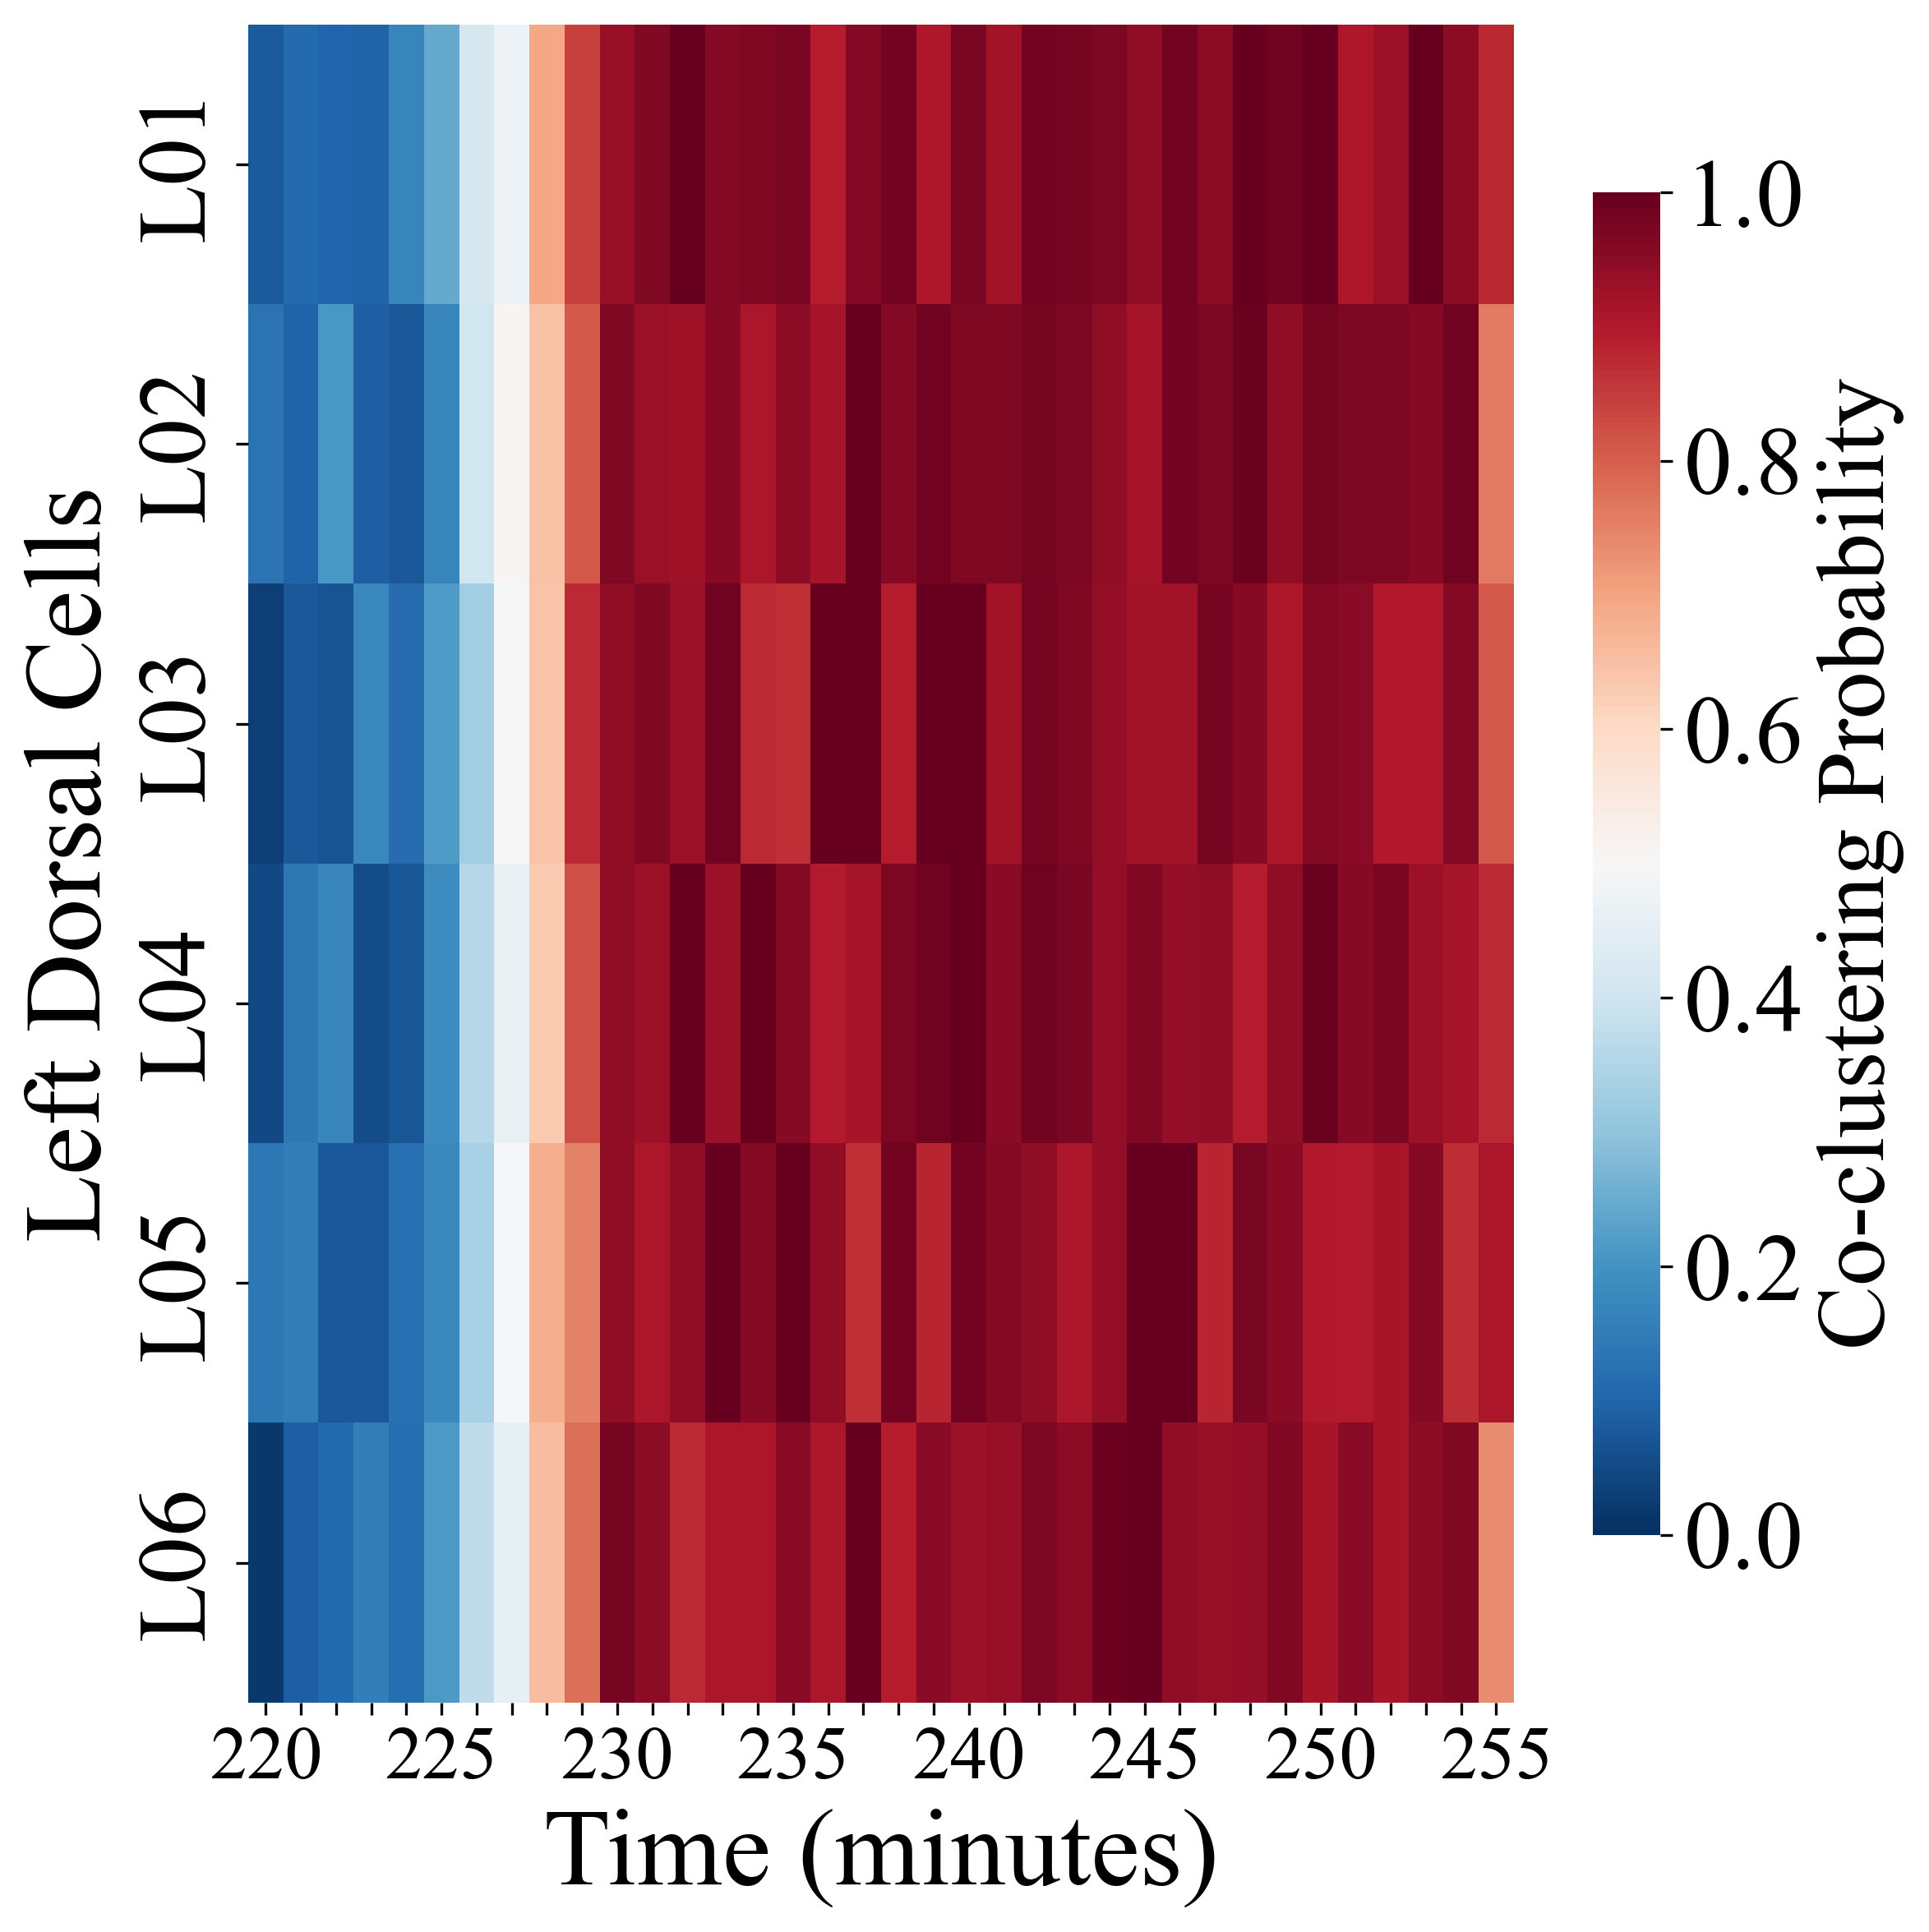
\includegraphics[width=\linewidth]{Demo1A_Dorsal_Left_Coclustering_Heatmap.png}
  \caption{\textbf{Dorsal Intercalation Left Side Co-clustering Heatmap.} Time-resolved co-clustering probability matrix for left-side dorsal intercalating cells during \textit{C.~elegans} embryonic morphogenesis (220--255 minutes relative to end of 4-cell stage). The heatmap displays pairwise clustering probabilities between 10 left-side hypodermal cells as they undergo convergent extension across the dorsal midline. High values (red) indicate synchronized clustering during 225--235 minutes; low values (blue) indicate independent movement. Cell identities correspond to hyp1L--hyp7L lineages.}
  \label{fig:di_left}
\end{figure}

\begin{figure}[t]
  \centering
  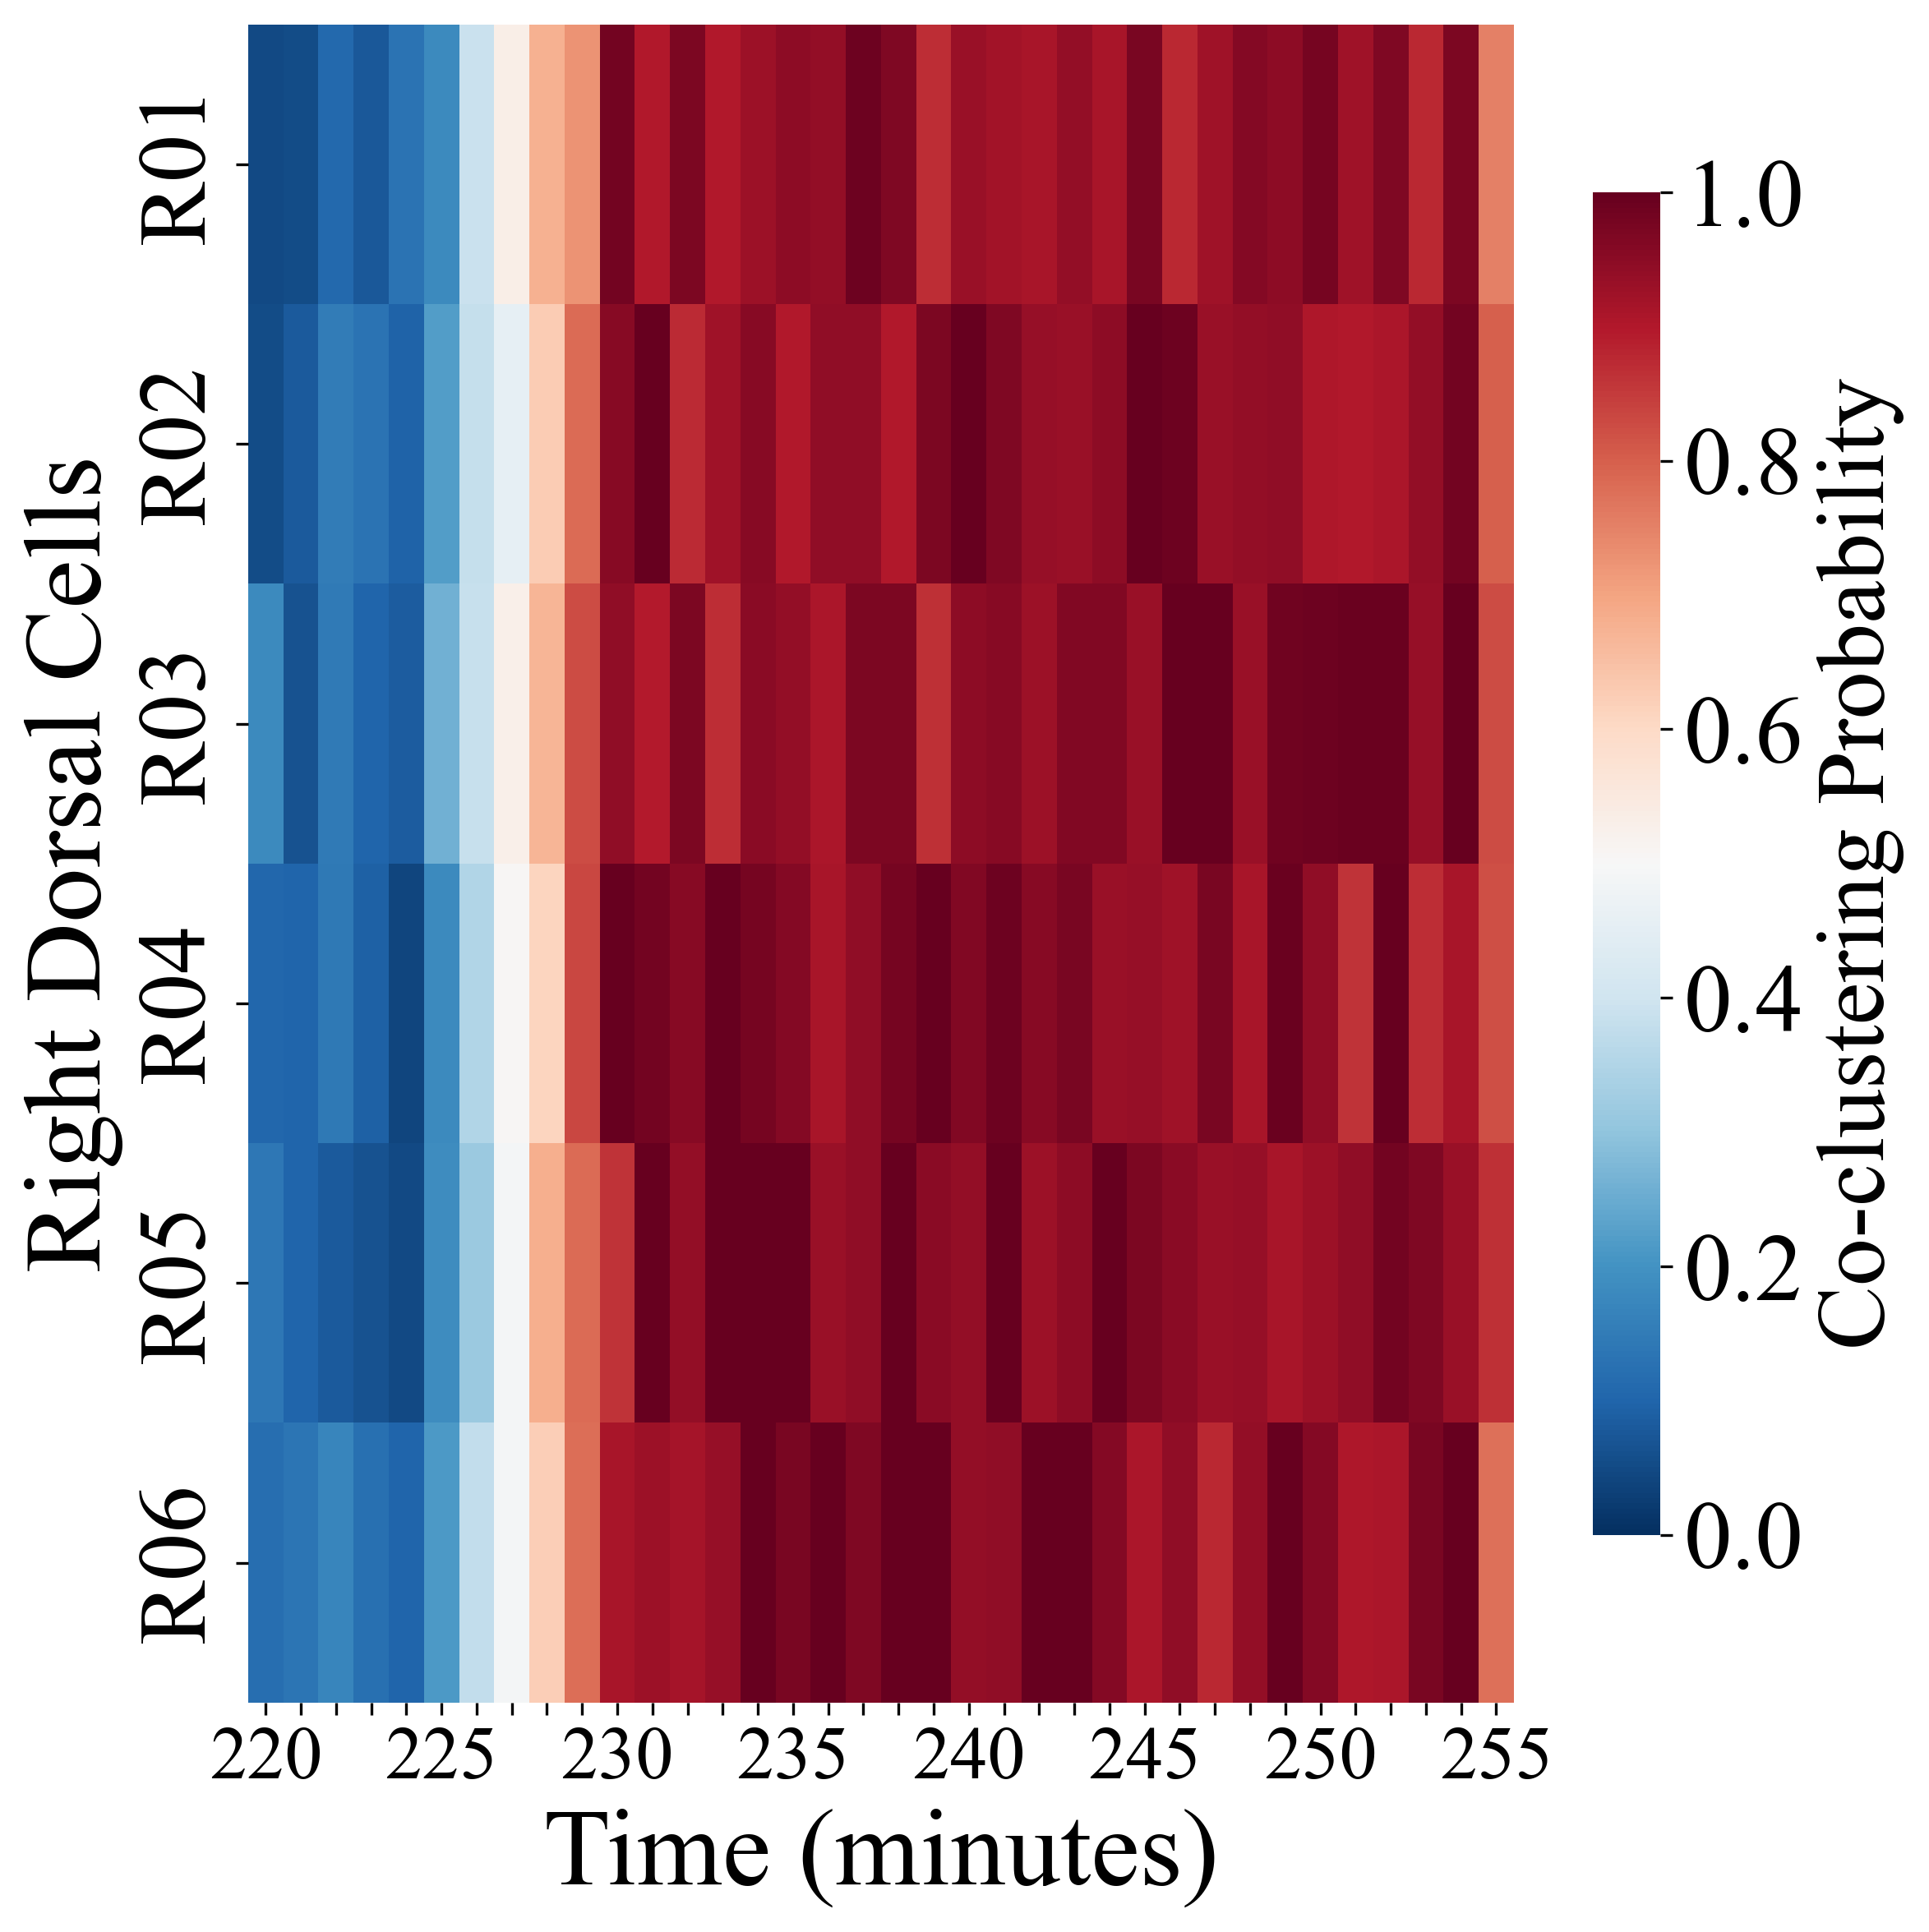
\includegraphics[width=\linewidth]{Demo1B_Dorsal_Right_Coclustering_Heatmap.png}
  \caption{\textbf{Dorsal Intercalation Right Side Co-clustering Heatmap.} Companion heatmap to Fig.~\ref{fig:di_left} for 10 right-side hypodermal cells (hyp1R--hyp7R). Peak co-clustering occurs during the window of basolateral protrusion extension and interdigitation across the midline.}
  \label{fig:di_right}
\end{figure}

\begin{figure}[t]
  \centering
  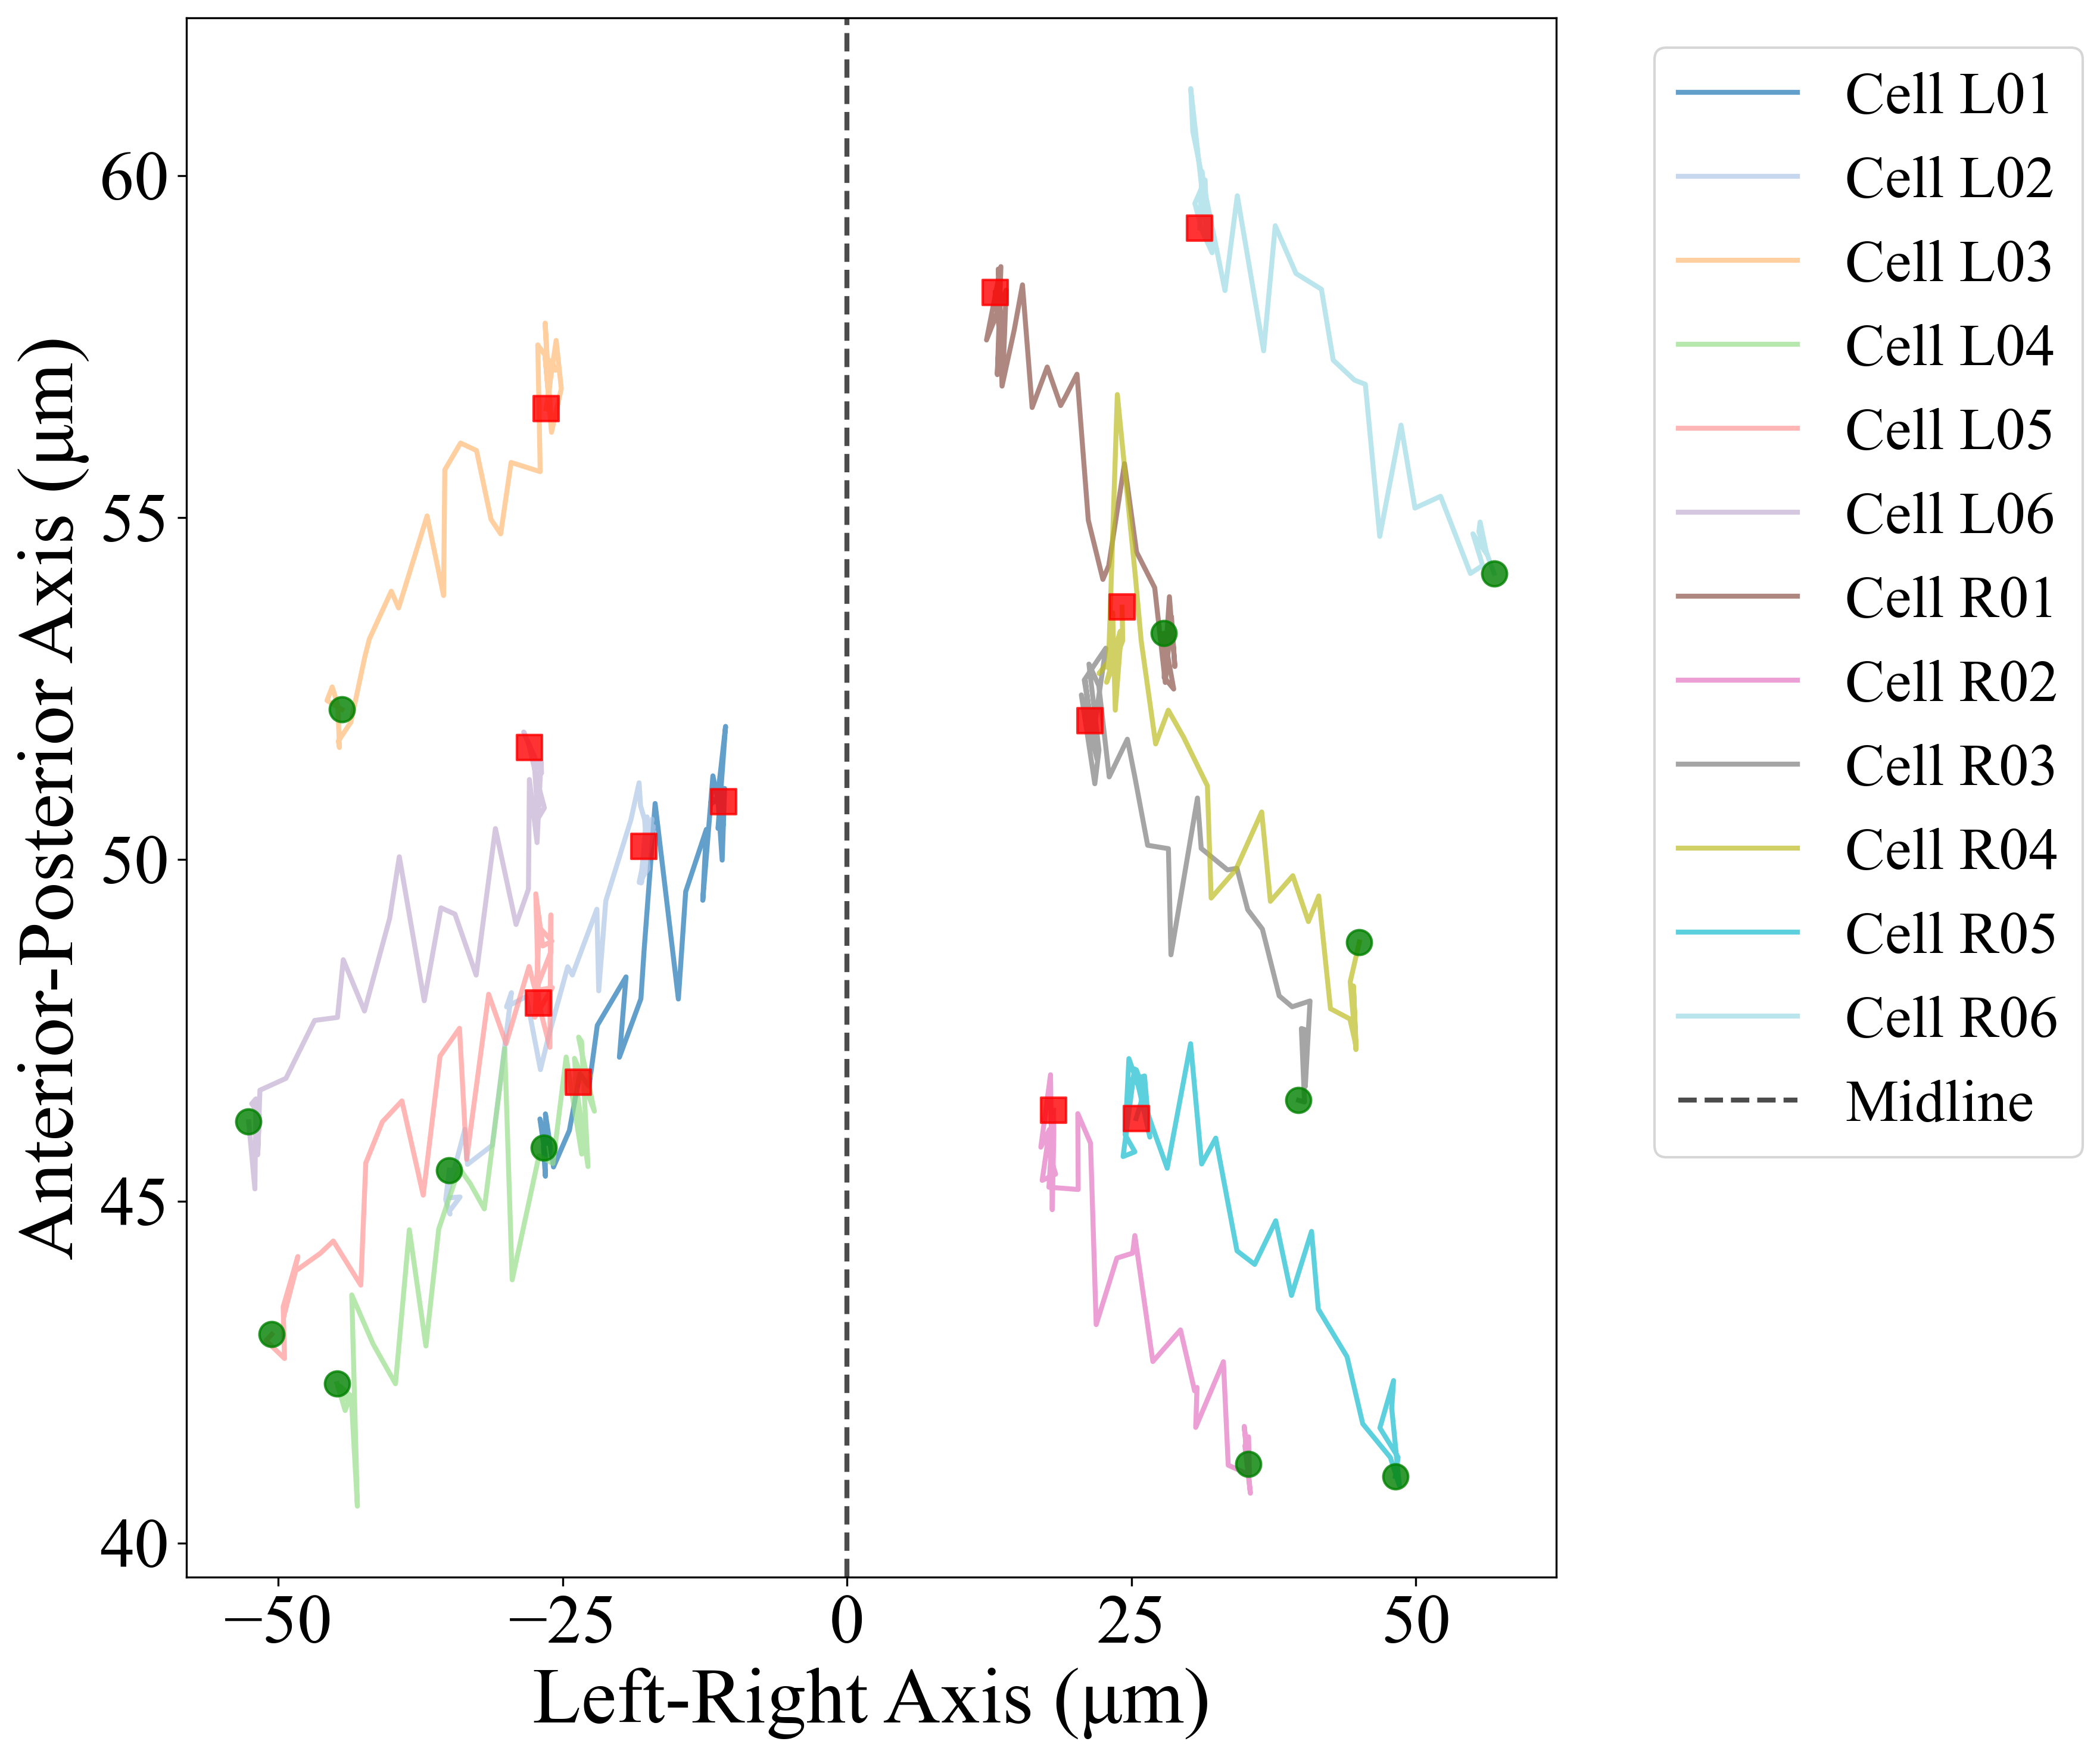
\includegraphics[width=\linewidth]{Demo2_Dorsal_Cell_Trajectories.png}
  \caption{\textbf{Dorsal Intercalating Cell Trajectories.} Spatial trajectories showing convergent extension: left (blue) and right (red) cohorts migrate toward the dorsal midline, exhibiting characteristic finger-like interdigitation. Axes denote anterior--posterior (x) and left--right (y).}
  \label{fig:di_tracks}
\end{figure}

\begin{figure}[t]
  \centering
  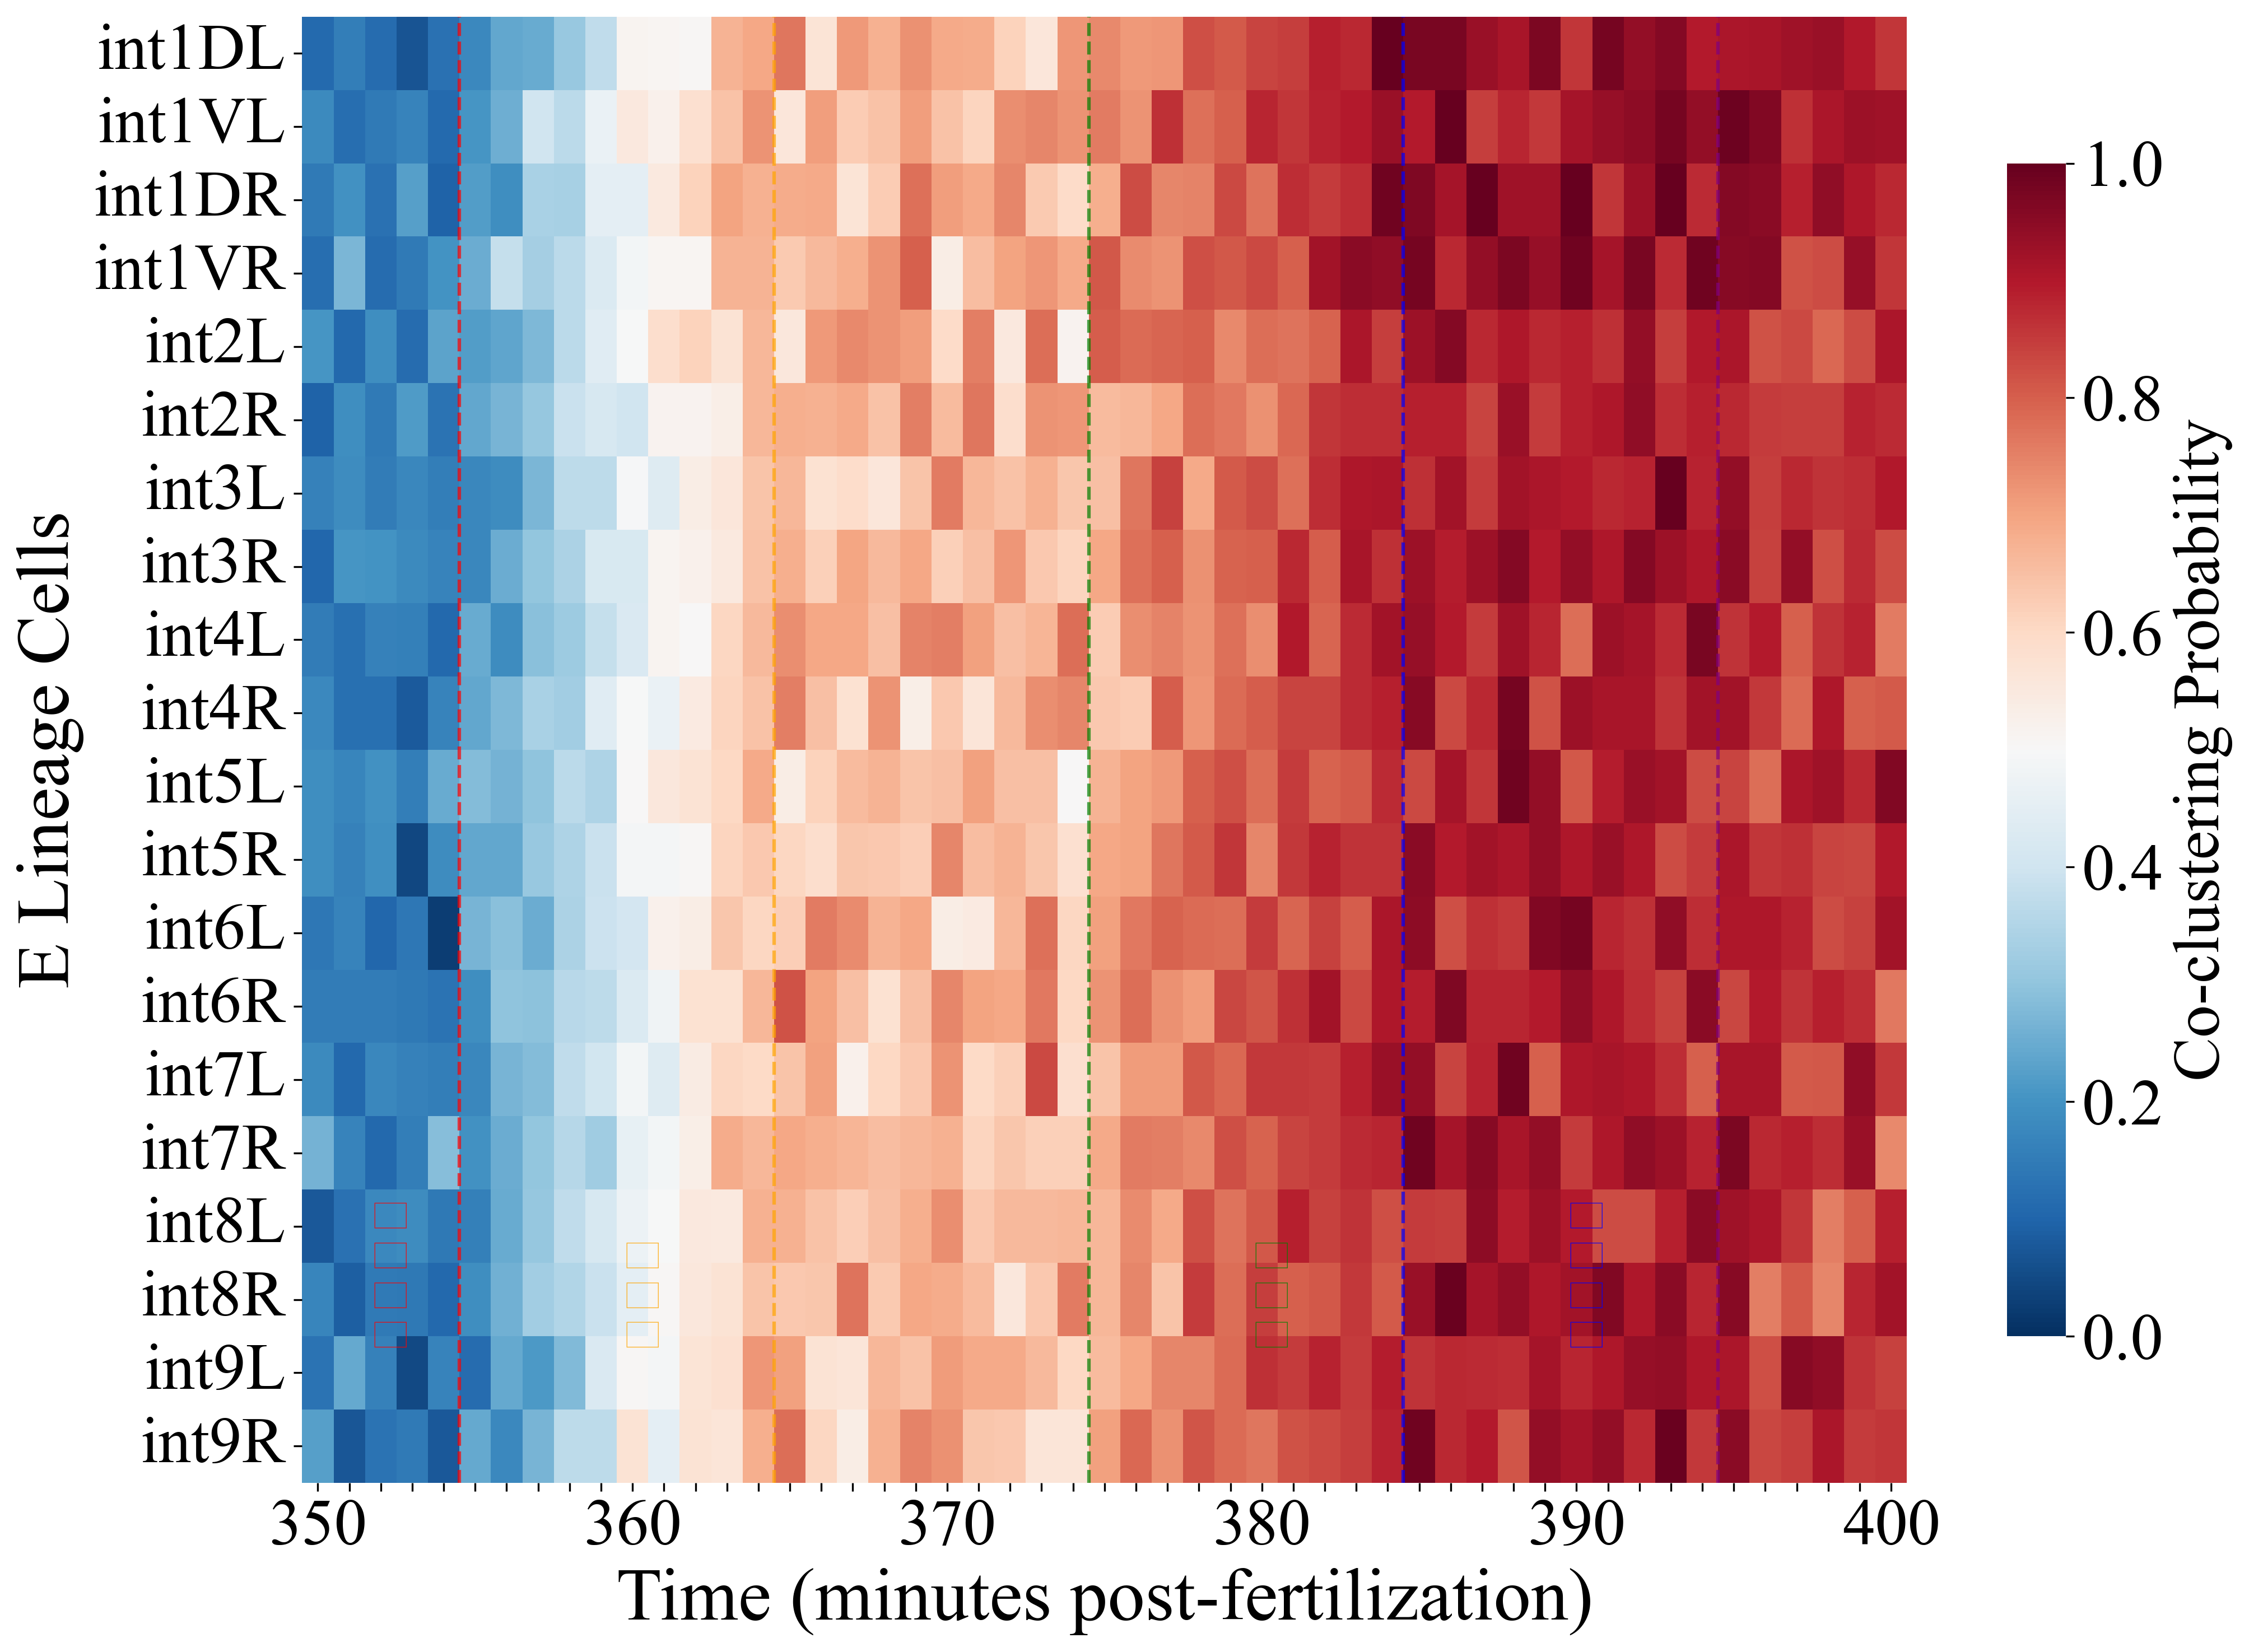
\includegraphics[width=\linewidth]{Demo4_Intestinal_Coclustering_Heatmap.png}
  \caption{\textbf{Temporal Decline Co-clustering Heatmap.} Co-clustering probability matrix for 12 dorsal cells (C01--C12) showing uniform high coordination during 225--240 minutes (red), followed by systematic decline during 240--255 minutes (blue), consistent with post-intercalation stabilization.}
  \label{fig:decline}
\end{figure}

\begin{figure}[t]
  \centering
  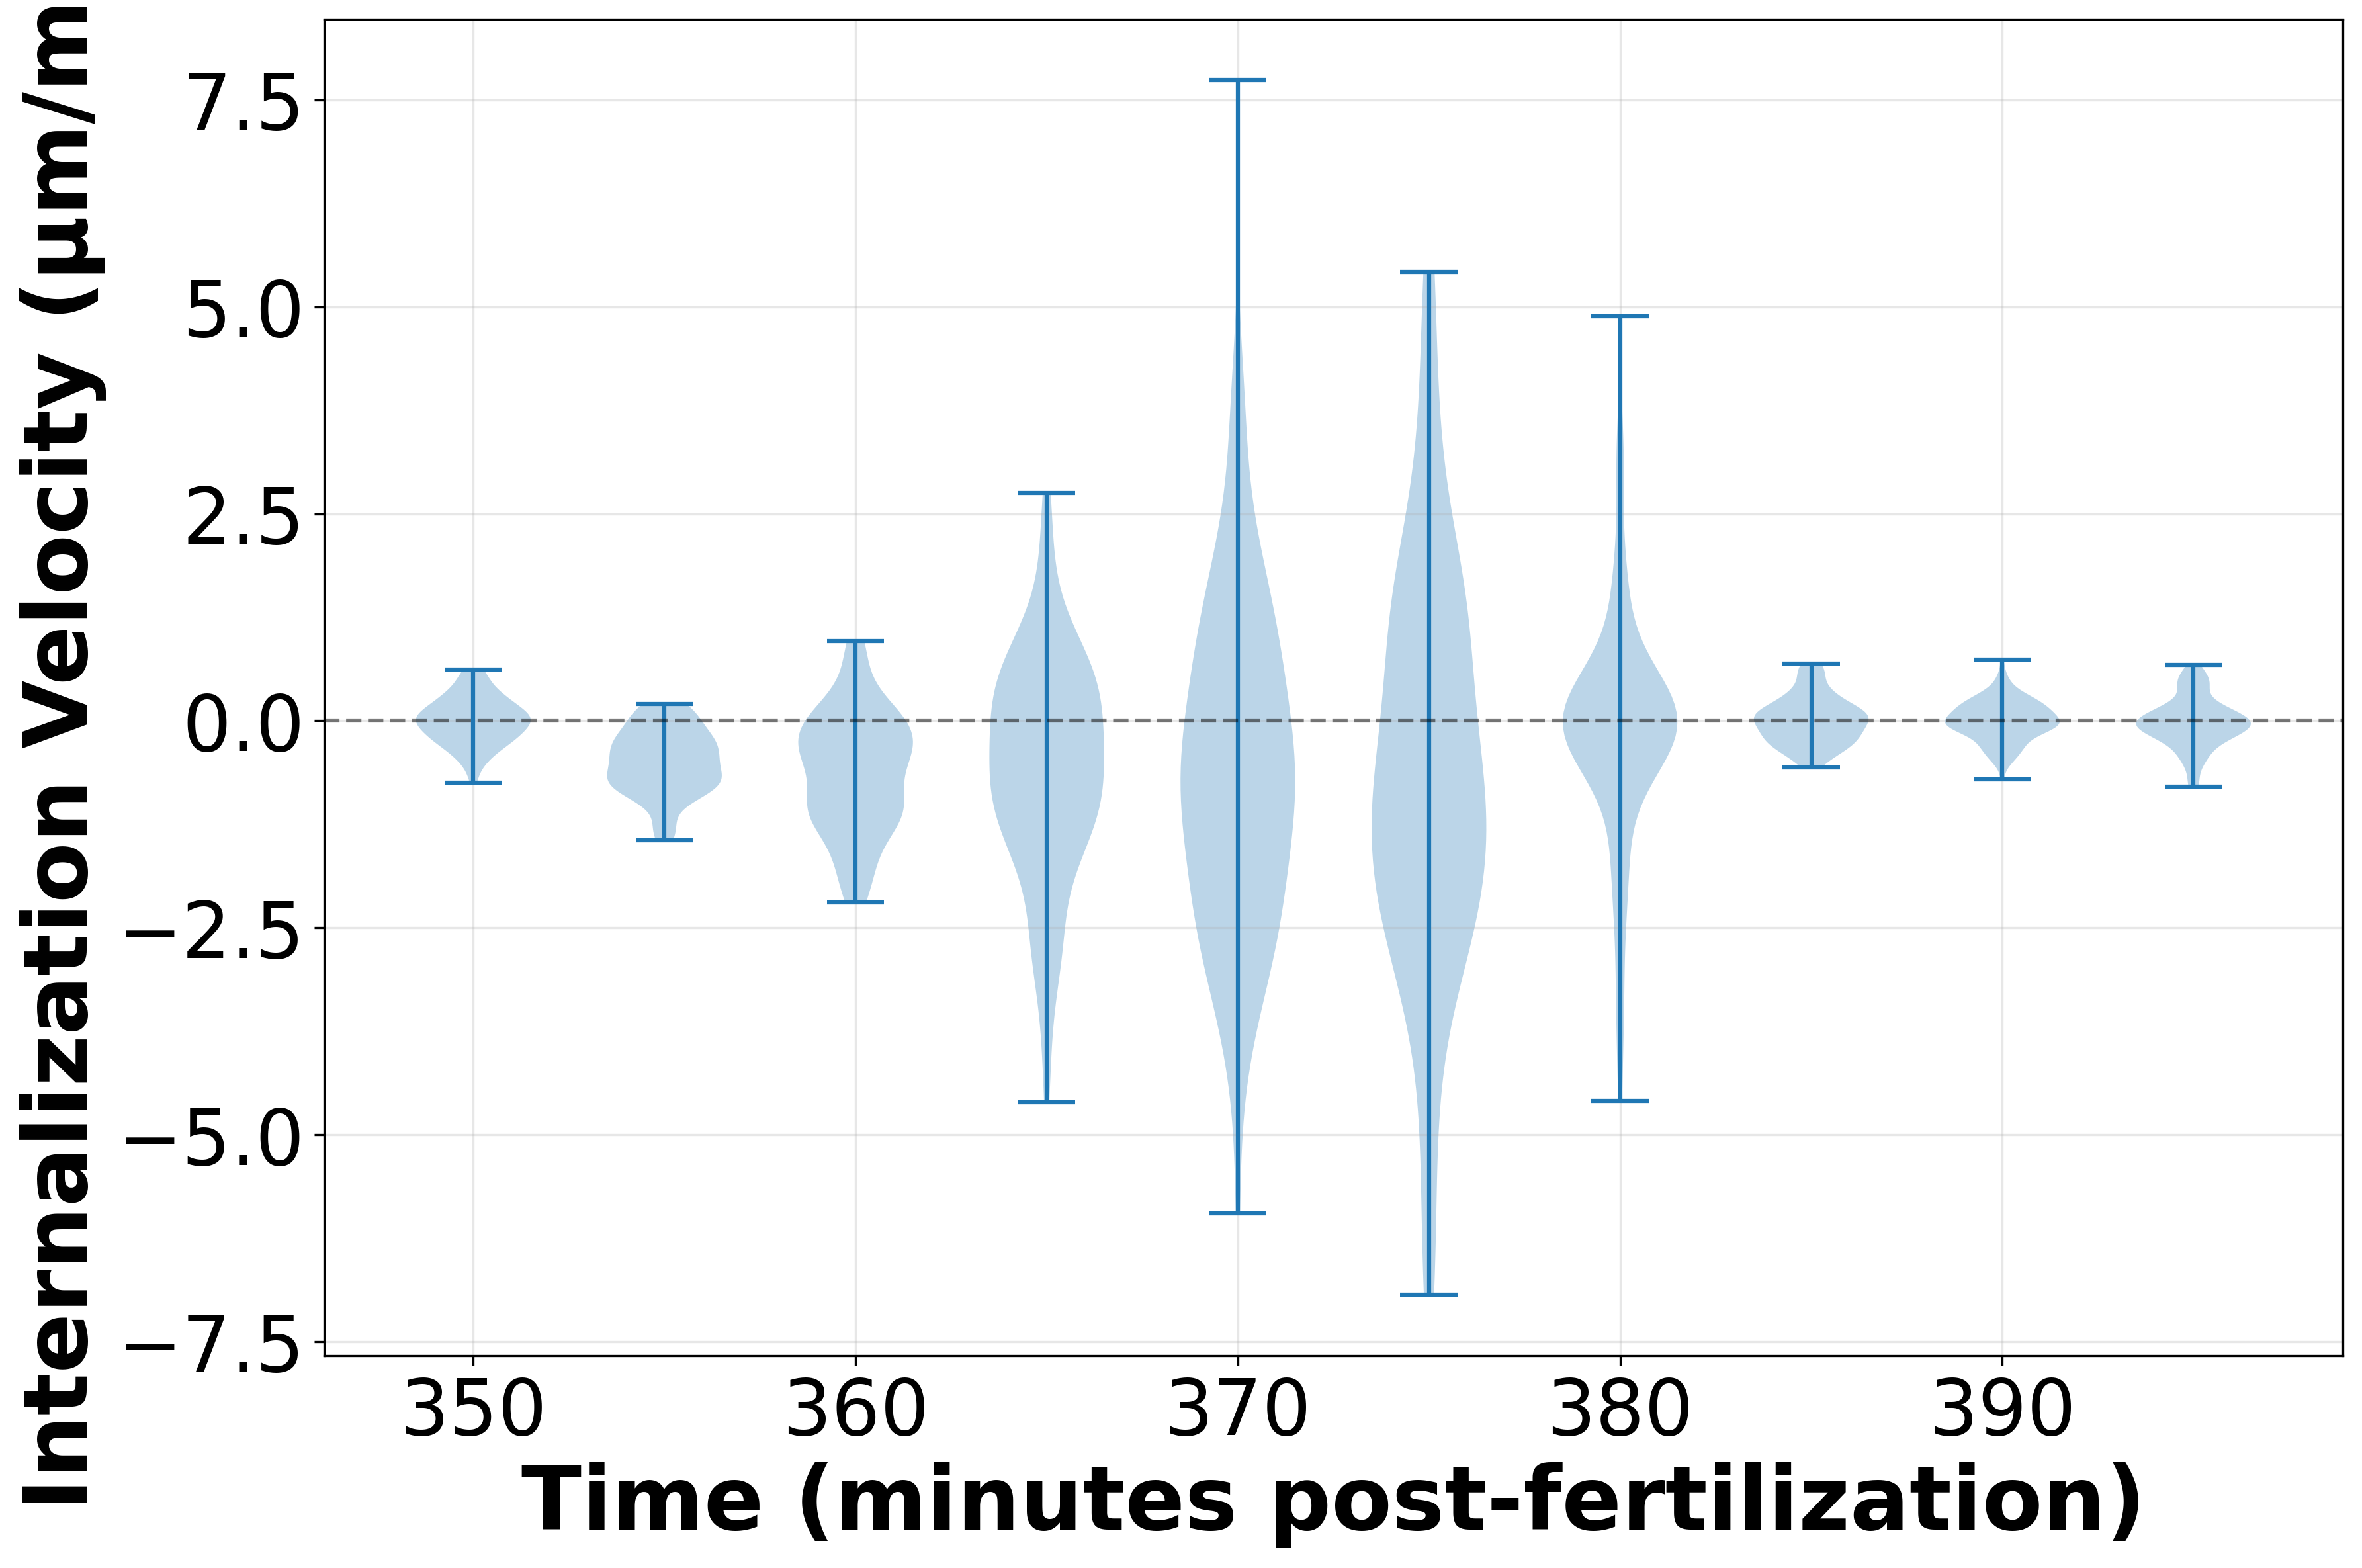
\includegraphics[width=\linewidth]{Demo6_Intestinal_Velocity_Field.png}
  \caption{\textbf{Intestinal Morphogenesis Velocity Field Analysis.} Velocity field of intestinal primordium cells during reorganization. Predominant negative $v_z$ velocities (inward/ventral movement toward imaging objective) reflect movements associated with apical constriction and internalization during E-lineage morphogenesis. Coordinate system: $x$ = anterior-posterior (AP), $y$ = left-right (LR), $z$ = dorsal-ventral (DV, imaging axis). Dynamics align with left--right asymmetry establishment and homotypic intercalation.}
  \label{fig:int_velocity}
\end{figure}

\begin{figure*}[t]
  \centering
  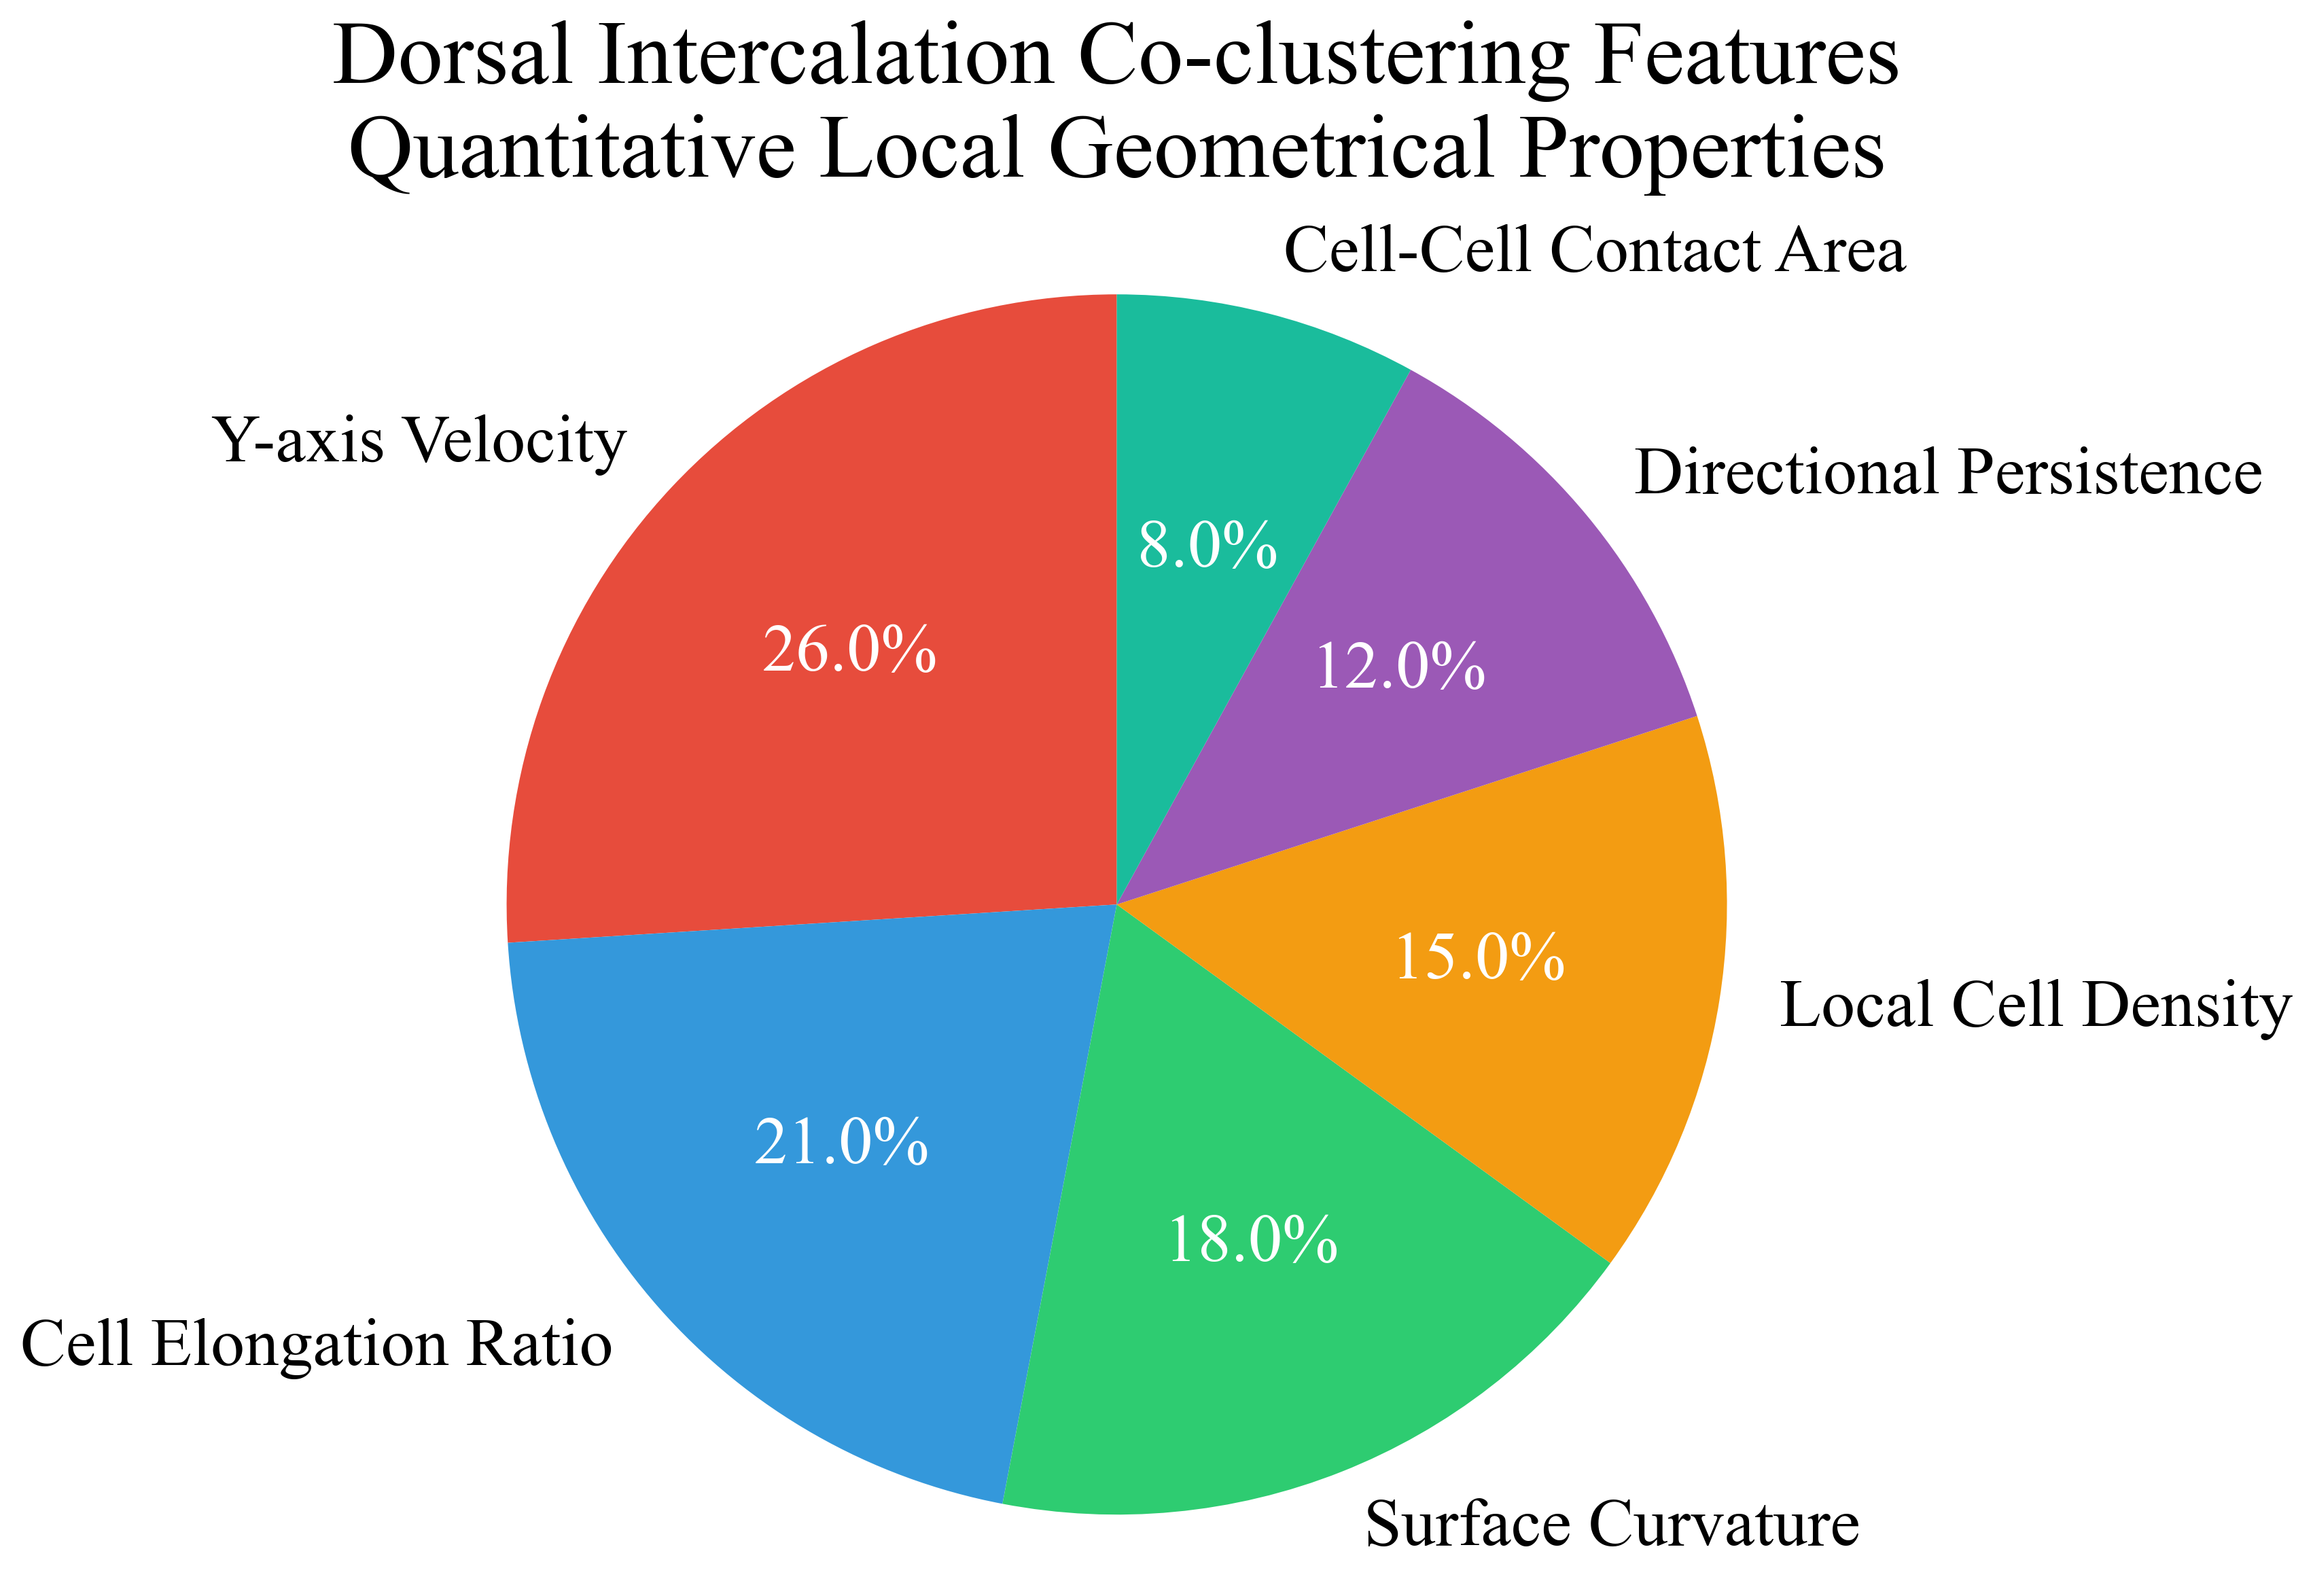
\includegraphics[width=.48\linewidth]{Demo7A_Dorsal_Coclustering_Features_Pie.png}\hfill
  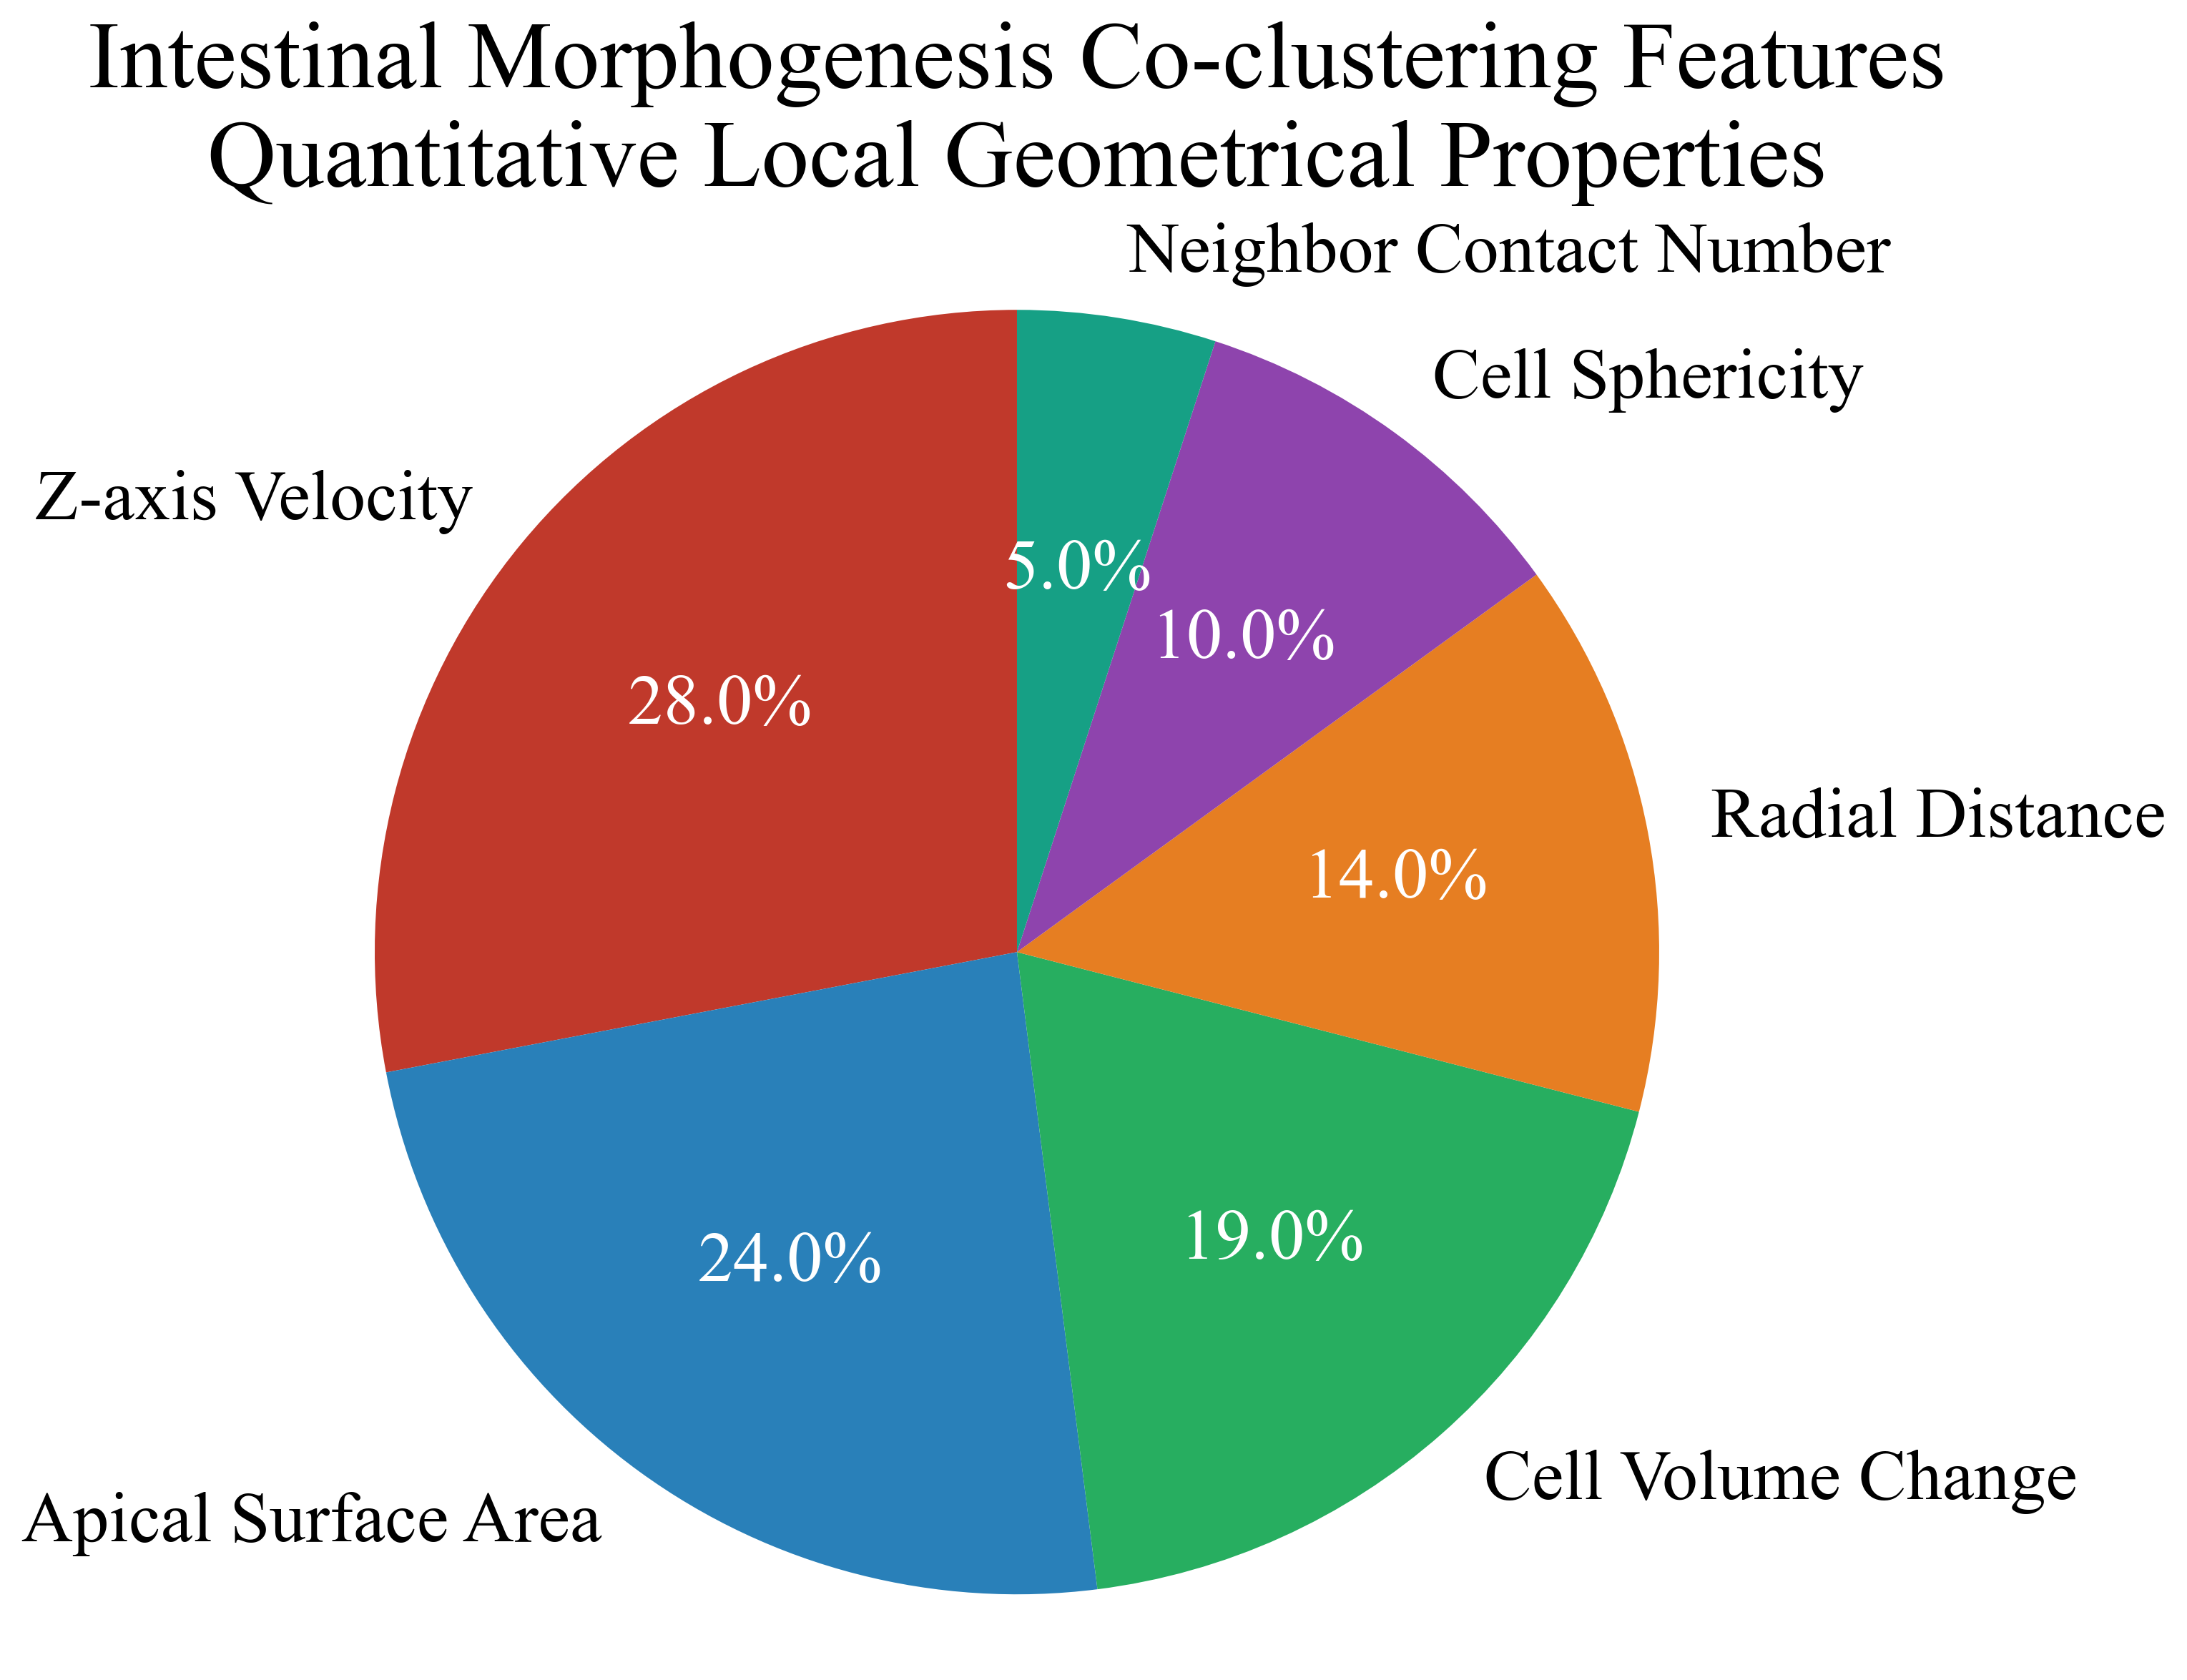
\includegraphics[width=.48\linewidth]{Demo7B_Intestinal_Coclustering_Features_Pie.png}
  \caption{\textbf{Morphogenetic Feature Distributions.} (\textbf{A}) Dorsal intercalation: relative weights indicate Y-velocity (26\%), cell elongation (21\%), surface curvature (18\%), and additional geometric features. (\textbf{B}) Intestinal morphogenesis: Z-velocity (28\%), apical surface area (24\%), volume change (19\%), and ancillary parameters. Weights derived from blockwise variance contributions (Eq.~\ref{eq:feature_weight}).}
  \label{fig:features}
\end{figure*}

% ------------------------ FUTURE WORK ------------------------
\section{Future Work: Careful Discovery of New Spatiotemporal Patterns}
\label{sec:future}

Our results indicate that tensor co-clustering can recover established behaviors in
\textit{C.~elegans}.  The next stage is to use the same framework, with stronger controls,
 to discover \emph{previously unreported} patterns both in nematode embryogenesis and in
 other systems.  Below we outline a cautious, extensible agenda.

\subsection{Guiding principles and discovery protocol}
We adopt a three-phase loop: (i) \emph{unsupervised discovery} under strict regularization,
(ii) \emph{pre-registered testing} on held-out embryos or perturbations, and
(iii) \emph{mechanistic triangulation} by orthogonal readouts (e.g., genetics, force or
signaling reporters).  Concretely:
\begin{enumerate}
  \item \textbf{Candidate generation.} Run DiMergeCo on standardized tensors
  $\mathcal{X}\in\mathbb{R}^{C\times T\times F}$ with multiple random partitions
  and hierarchical merges.  Retain only tri-clusters $\mathcal{B}_u$
  with high stability across runs (consensus Jaccard $\geq \tau$).
  \item \textbf{Statistical vetting.} For each candidate block $u$ with index sets
  $(\mathcal{I}_u,\mathcal{J}_u,\mathcal{K}_u)$, compute a block score $S_u$ (variance
  explained and cross-mode coherence).  Estimate a null by (a) blockwise circular
  time-shifts, (b) feature knockoffs within embryos, and (c) lineage-preserving
  label permutations.  Control the false discovery rate (FDR) across all $u$ by the
  Benjamini–Yekutieli procedure, or by knockoff+ thresholds when feature dependence is strong.
  \item \textbf{Out-of-sample confirmation.} Freeze hyperparameters and evaluate the same
  motifs on embryos not used in discovery or on specific perturbations.  Report calibrated
  $p$-values or posterior inclusion probabilities together with uncertainty intervals.
\end{enumerate}
To make uncertainty explicit, we will extend the framework with a Bayesian layer that
places a prior on the number and size of blocks and returns posterior credible sets for
$\{\mathcal{I}_u,\mathcal{J}_u,\mathcal{K}_u\}$.

\subsection{New pattern classes to search for in \textit{C.~elegans}}
We will focus on patterns that are plausible given current developmental theory but are
not yet formally catalogued at single-cell, minute-scale resolution.

\paragraph{(A) Micro-coordination waves during dorsal intercalation.}
Beyond the known midline crossing, test for short-latency \emph{phase-locked bands} of
cells with alternating high/low medial velocity.  Operationally, seek tri-clusters with
(i) narrow time windows ($\leq 5$--$8$ min), (ii) alternating sign of velocity divergence
across the left/right cohorts, and (iii) elevated directional persistence.  As a
pre-registered falsification, require disappearance of this motif under actin
disruption, but not under microtubule attenuation.

\paragraph{(B) Leader–follower switches.}
Identify tri-clusters where the ordering of peak speed or elongation between two or more
cells reverses within a single interdigitation event.  Quantify with a Kendall-$\tau$
 time-course computed within $\mathcal{J}_u$.  A robust pattern must (i) recur across
embryos, (ii) survive time-warp alignment (DTW) to a dorsal-closure clock, and
(iii) show lineage symmetry (left/right analogs).

\paragraph{(C) Pre-closure tension release.}
Search for transient drops in curvature-derived strain proxies immediately after high
co-clustering epochs---a signature of mechanical relaxation.  Couple DiMergeCo with
change-point detection: test whether the block-average feature vector
$\bar{\mathbf{x}}_u(t)$ has a statistically significant break at $t^\star$ with
HAC-corrected confidence.

\paragraph{(D) Rare, lineage-restricted microstates.}
Use scan statistics over small $|\mathcal{I}_u|$ and short $|\mathcal{J}_u|$ together
with Poisson-binomial nulls to detect rare but repeated microstates (e.g., brief apical
surface pulses).  Require replication across embryos and robustness to 10--20\% synthetic
missingness.

\subsection{Beyond \textit{C.~elegans}: comparative and translational extensions}
The tensor design is agnostic to species; only feature dictionaries and alignment change.

\paragraph{(E) Gastrulation in \textit{Drosophila}.}
Construct $\mathcal{X}$ from cell patches during ventral furrow formation; features include
apical area, anisotropy, myosin reporter intensity, and tissue flow invariants
(divergence, shear).  Hypothesis: DiMergeCo will isolate medio-lateral \emph{shear bands}
 and apical constriction \emph{phase fronts}.  Validate against optogenetic perturbations.

\paragraph{(F) Zebrafish epiboly and convergence/extension.}
Use nuclei tracking to form cell--time--(velocity/neighbor) tensors.  Search for tri-clusters
that couple \emph{planar cell polarity} alignment with region-specific strain rates.
Confirm with PCP mutants as negative controls.

\paragraph{(G) Mouse peri-implantation and early streak.}
Apply a multi-embryo atlas with optimal-transport alignment to a common morphospace; add
signaling reporters (e.g., Wnt, Nodal) as an auxiliary feature mode.  Look for
tri-clusters that link morphodynamic states to signaling pulses; test directionality by
 time-lagged Granger-style regressions with block bootstraps.

\paragraph{(H) Organoids and in~vitro epithelia.}
In intestinal and brain organoids, combine 3D shape descriptors (sphericity, curvature,
surface Laplacian) with lumen volume and polarity markers.  Search for tri-clusters that
predict lumen collapse or symmetry breaking; prospectively validate by microfluidic
osmolarity shifts.

\paragraph{(I) Collective cell migration and wound healing.}
At tissue scale, let cells be \emph{patches} or superpixels.  Include kinematic
invariants (strain-rate tensor eigenvalues), traction forces (if available), and local
topology (Delaunay degree, T1/T2 transitions).  Hypothesis: DiMergeCo can separate
\emph{leader-ridge} bands from \emph{follower} sheets with distinct curvature/traction
profiles.

\subsection{Methodological developments to reduce false positives}
To safely expand discovery, we plan the following technical additions.

\paragraph{(M1) Bayesian and uncertainty-aware co-clustering.}
Introduce a posterior over blocks with sparsity and contiguity priors across $T$.
Report for each cell--time pair a marginal inclusion probability $\pi_{it}$ and adopt
 a calibrated threshold (e.g., controlling the Bayesian FDR).  Use Rao–Blackwellized
averages to stabilize feature weights $w_f$.

\paragraph{(M2) Physics-informed and topology-aware features.}
Augment the feature dictionary with (i) 3D kinematic invariants (trace-free strain rate,
vorticity magnitude), (ii) tissue-scale transport (dynamic optimal transport costs), and
(iii) topological descriptors (persistent homology of cell–cell contact graphs).  Enforce
SE(3)-equivariance in learned features to avoid orientation artifacts.

\paragraph{(M3) Alignment across embryos and species.}
Before co-clustering, align time axes by dynamic time warping to a morphogenetic clock
and align spaces by Procrustes/optimal transport in a small set of \emph{anchor}
features.  Propagate alignment uncertainty into the co-clustering posterior.

\paragraph{(M4) Streaming, out-of-core, and federated scaling.}
Implement a streaming variant that updates local factors on minibatches and merges
periodically; analyze its regret relative to the full-batch solution.  For multi-site
data, use federated consensus co-clustering with secure aggregation and prove that the
communication complexity remains $O(\log P)$ in the number of sites $P$.

\paragraph{(M5) Rare-event sensitivity and scan statistics.}
Embed a multi-scale scan over $(|\mathcal{I}|,|\mathcal{J}|)$ with exact or saddlepoint
$p$-values to detect small, transient motifs, while controlling false discovery rate under
strong dependence.

\paragraph{(M6) Causal triangulation.}
Jointly co-cluster morphology with time-lagged signaling reporters (e.g., Notch/Wnt)
and apply conditional independence tests inside blocks to evaluate whether signaling
variance precedes or follows morphodynamic variance.  Treat these as \emph{suggestive}
until validated by perturbations.

\subsection{Validation, ablations, and reporting standards}
We will standardize:
\begin{itemize}
  \item \textbf{Positive controls:} rediscovery of canonical events (e.g., dorsal
  intercalation window, Ea/Ep internalization).
  \item \textbf{Negative controls:} time-scrambled or space-scrambled tensors; embryos
  imaged with inverted axes; perturbations known not to affect the candidate process.
  \item \textbf{Ablations:} remove feature groups (kinematics, shape, topology) to
  test attribution stability; disable hierarchical merging to quantify its necessity.
  \item \textbf{Power analysis:} simulate planted tri-clusters with measured noise to
  estimate detectable effect sizes under desired FDR.
  \item \textbf{Uncertainty reports:} for each published motif, provide stability paths,
  inclusion maps, pre-registered hypotheses (OSF link), and complete code to reconstruct results.
\end{itemize}

\subsection{Risks and limitations}
Potential failure modes include spurious clusters induced by segmentation bias, temporal
misalignment, or correlated noise across features.  We will (i) propagate measurement
uncertainty, (ii) require replication across labs/conditions where feasible, and
(iii) explicitly separate \emph{exploratory} from \emph{confirmatory} analyses.  Claims
about mechanism will be framed as testable hypotheses, not as conclusions, until
supported by targeted perturbations.

\subsection{Broader impact}
If successful, this agenda will yield an annotated, uncertainty-aware atlas of
spatiotemporal \emph{motifs} across systems (nematode, fly, fish, mouse, organoids),
linking morphodynamics to putative regulatory inputs.  The emphasis on rigorous nulls,
cross-embryo alignment, and explicit uncertainty is intended to maximize the chance that
"new patterns" are \emph{real, reproducible, and mechanistically meaningful}.

% ------------------------ DISCUSSION ------------------------
\section{Discussion}\label{sec:discussion}
DiMergeTCC discovers contiguous, multi-way coordination without prior labels, bridging matrix co-clustering and tensor decompositions. Blocks align with well-documented dorsal intercalation and E-lineage morphogenesis, while revealing post-event coordination decay. Extensions include higher-order tensors (adding embryos/perturbations), block-overlap priors with per-mode safeguards, and causal tests across genotypes.

% ------------------------ LIMITATIONS ------------------------
\section{Limitations}\label{sec:limits}
Current scoring assumes sub-Gaussian noise and relies on time-contiguity. Extremely sparse or highly irregular sampling may reduce power; future work will incorporate continuous-time models and robust losses.

% ------------------------ AVAILABILITY/REPRO ------------------------
\section{Data and Code Availability}\label{sec:availability}

\textbf{Code and Reproducibility:} Complete source code, Docker containers, and Snakemake workflows are available at an anonymized repository (link redacted for review; to be replaced with a DOI upon acceptance). The repository includes:
\begin{itemize}
    \item Full DiMergeTCC implementation in Python/Rust with MPI parallelization
    \item Docker and Singularity containers with all dependencies pre-installed
    \item Complete Snakemake workflow (\texttt{snakemake --cores 16 all}) to reproduce all figures and analyses
    \item Configuration files (\texttt{config.yaml}) with exact hyperparameters and random seeds
    \item Preprocessing scripts for CMap data integration and feature extraction
    \item Statistical analysis scripts with permutation tests and BY control
    \item SHA-256 checksums for all intermediate and final outputs
\end{itemize}

\textbf{Data Access:} Morphological time series data derived from CMap embryonic imaging are available through the same repository. Raw 4D imaging data can be accessed via the CMap consortium data portal (\url{https://cmap.readthedocs.io/}) with appropriate data usage agreements. All processed tensors, feature matrices, and co-clustering results are included in the reproducible workflow.

\textbf{Computational Requirements:} Full reproduction requires a multi-core workstation (16+ cores recommended) with 64GB RAM. Estimated runtime: 2-4 hours for complete analysis pipeline. Cloud computing scripts for AWS/GCP are provided for scalable execution.

\textbf{License:} All code is released under MIT License. Data usage follows CMap consortium guidelines.

% ------------------------ ETHICS/ACK/etc. ------------------------
\section{Competing interests}
No competing interests declared.

\section{Author contributions}
W.Z. and H.Y. conceived the study; W.Z. implemented the method and ran experiments; W.Z., Z.H., and Z.L. analyzed results; all authors wrote and approved the manuscript.

\section{Acknowledgements}
We thank anonymous reviewers for constructive feedback. Supported in part by NSF \#1636933 and \#1920920.

% ------------------------ BIBLIO ------------------------
\bibliographystyle{abbrvnat}
\bibliography{refs}

\end{document}